% =============================================================================
%  Informe: Bomberman Concurrente en C con POSIX
%  Compilar desde la carpeta informe/:   pdflatex informe.tex  (dos veces)
%  Las figuras y los numeros de las tablas los genera experimentos/graficos.py
%  a partir de los CSV de experimentos/datos/ (que produce experimentos/run.sh).
% =============================================================================
\documentclass[11pt,a4paper]{article}

\usepackage[T1]{fontenc}
\usepackage[utf8]{inputenc}
\usepackage[spanish,es-noshorthands,es-tabla]{babel}
\usepackage{newtxtext}
\usepackage[varqu]{inconsolata}
\usepackage[a4paper,top=2.5cm,bottom=2.5cm,left=2.5cm,right=2.5cm]{geometry}
\usepackage{graphicx}
\usepackage{xcolor}
\usepackage{tikz}
\usetikzlibrary{positioning,arrows.meta,fit,backgrounds,calc,shapes.geometric,babel}
\usepackage{booktabs,tabularx,array,multirow}
\usepackage[font=small,labelfont=bf,labelsep=period]{caption}
\usepackage{float}
\usepackage{enumitem}
\usepackage{pdflscape}
\usepackage{needspace}
\usepackage[hidelinks]{hyperref}
\usepackage{url}

% ---- colores (mismos que las figuras) ----
\definecolor{colP0}{HTML}{3D5A80}
\definecolor{colP1}{HTML}{2A78D6}
\definecolor{colP2}{HTML}{EB6834}
\definecolor{colP3}{HTML}{C98500}
\definecolor{colP4}{HTML}{6250D6}
\definecolor{colMem}{HTML}{1B8A62}

\setlist{itemsep=2pt,topsep=4pt}
\setlength{\parskip}{4pt}
\renewcommand{\arraystretch}{1.18}
\newcolumntype{Y}{>{\raggedright\arraybackslash}X}
\newcommand{\cod}[1]{\texttt{#1}}
\renewcommand{\_}{\textunderscore\allowbreak}
\setlength{\emergencystretch}{2.5em}

% ---- datos de la portada (completar) ----
\newcommand{\curso}{Sistemas Computacionales (IS2021)}
\newcommand{\docente}{(completar)}
\newcommand{\repo}{https://github.com/JoelxD12O/bomberman-concurrente}

% ---- numeros de los experimentos (generados) ----
% Generado por experimentos/graficos.py: no editar a mano
\newcommand{\NJuegoTexto}{\textbf{Resultado.} En los 6 escenarios, las 1\,800 corridas produjeron exactamente una salida distinta por caso: el mismo orden de turnos, las mismas explosiones en los mismos ticks y el mismo resultado final. En estos escenarios ninguna carrera altera el resultado. Esto no prueba que no existan: la Familia~2c muestra una carrera real que estos casos no ejercitan.}
\newcommand{\NTrackerTexto}{La partida correcta termina con 2 vidas. Con el código del PR~\#21 tal cual, sin ninguna amplificación, \textbf{el 4.0\,\% de las corridas (12 de 300) perdió el choque} y terminó con 3 vidas: la carrera ocurría en el código de P2 del PR~\#21. Con el retardo de 2~ms el detector compara casi siempre contra la copia anterior, y solo el 0.0\,\% de las corridas detecta el choque. Con la corrección (y el mismo retardo), lo detecta el 100.0\,\%. En los casos de prueba del repositorio la carrera no se ve porque, en \cod{caso\_demo}, Bomberman lleva varios turnos quieto cuando lo alcanza el enemigo: la copia vieja y la nueva coinciden. Por eso la validación de la Tabla~\ref{tab:juego} no podía detectarla. La corrección es la que hoy usa \cod{main} (PR~\#26).}
\newcommand{\NcincoBugCpu}{97}
\newcommand{\NcincoBugLimpias}{0.0}
\newcommand{\NcincoBugMax}{192\,560}
\newcommand{\NcincoBugMaxPct}{96.3}
\newcommand{\NcincoBugMedia}{180\,037}
\newcommand{\NcincoBugMediaPct}{90.0}
\newcommand{\NcincoBugMem}{2\,032}
\newcommand{\NcincoBugMin}{157\,648}
\newcommand{\NcincoBugSd}{3\,773}
\newcommand{\NcincoBugTiempo}{0.0414}
\newcommand{\NcincoN}{500}
\newcommand{\NcincoOkCpu}{119}
\newcommand{\NcincoOkLimpias}{100.0}
\newcommand{\NcincoOkMax}{0}
\newcommand{\NcincoOkMem}{2\,096}
\newcommand{\NcincoOkTiempo}{0.1631}
\newcommand{\NcuatroBugCpu}{13}
\newcommand{\NcuatroBugLimpias}{0.2}
\newcommand{\NcuatroBugMax}{3\,512}
\newcommand{\NcuatroBugMaxPct}{1.8}
\newcommand{\NcuatroBugMedia}{368}
\newcommand{\NcuatroBugMediaPct}{0.2}
\newcommand{\NcuatroBugMem}{1\,776}
\newcommand{\NcuatroBugMin}{0}
\newcommand{\NcuatroBugSd}{377}
\newcommand{\NcuatroBugTiempo}{0.0100}
\newcommand{\NcuatroN}{500}
\newcommand{\NcuatroOkCpu}{116}
\newcommand{\NcuatroOkLimpias}{100.0}
\newcommand{\NcuatroOkMax}{0}
\newcommand{\NcuatroOkMem}{1\,776}
\newcommand{\NcuatroOkTiempo}{0.0398}
\newcommand{\NdosBugCpu}{86}
\newcommand{\NdosBugLimpias}{0.0}
\newcommand{\NdosBugMax}{98}
\newcommand{\NdosBugMedia}{17.0}
\newcommand{\NdosBugMem}{1\,904}
\newcommand{\NdosBugMin}{1}
\newcommand{\NdosBugSd}{13.2}
\newcommand{\NdosBugTiempo}{0.0209}
\newcommand{\NdosN}{500}
\newcommand{\NdosOkCpu}{77}
\newcommand{\NdosOkLimpias}{100.0}
\newcommand{\NdosOkMem}{1\,904}
\newcommand{\NdosOkTiempo}{0.0252}
\newcommand{\NequiBugCpu}{120}
\newcommand{\NequiBugMax}{1\,439}
\newcommand{\NequiBugMedia}{487}
\newcommand{\NequiBugMediaPct}{1.9}
\newcommand{\NequiBugMem}{1\,904}
\newcommand{\NequiBugSd}{203}
\newcommand{\NequiBugTiempo}{1.0575}
\newcommand{\NequiN}{200}
\newcommand{\NequiOkCpu}{99}
\newcommand{\NequiOkMax}{0}
\newcommand{\NequiOkMem}{1\,904}
\newcommand{\NequiOkTiempo}{1.8606}
\newcommand{\NequiPeorMax}{25\,739}
\newcommand{\NequiPeorMin}{24\,300}
\newcommand{\NequiRepA}{24\,734}
\newcommand{\NequiRepB}{25\,064}
\newcommand{\NequiRepC}{25\,197}
\newcommand{\NequiRepD}{25\,005}
\newcommand{\NequiRepDes}{463}
\newcommand{\NequiRepPct}{1.9}
\newcommand{\NjuegoN}{300}
\newcommand{\NseisABugCierra}{0}
\newcommand{\NseisABugCpu}{0}
\newcommand{\NseisABugMem}{1\,892}
\newcommand{\NseisABugTiempo}{1.0007}
\newcommand{\NseisAN}{50}
\newcommand{\NseisAOkCierra}{100}
\newcommand{\NseisAOkCpu}{74}
\newcommand{\NseisAOkMem}{1\,892}
\newcommand{\NseisAOkMs}{3.8}
\newcommand{\NseisAOkTiempo}{0.0044}
\newcommand{\NseisBBugCierra}{0}
\newcommand{\NseisBBugCpu}{4}
\newcommand{\NseisBBugMem}{1\,968}
\newcommand{\NseisBBugTiempo}{1.0002}
\newcommand{\NseisBN}{50}
\newcommand{\NseisBOkCierra}{100}
\newcommand{\NseisBOkCpu}{81}
\newcommand{\NseisBOkMem}{1\,968}
\newcommand{\NseisBOkMs}{7.2}
\newcommand{\NseisBOkTiempo}{0.0075}
\newcommand{\NsieteAAhoraCierra}{100}
\newcommand{\NsieteAAhoraCpu}{52}
\newcommand{\NsieteAAhoraMem}{1\,664}
\newcommand{\NsieteAAhoraTiempo}{0.066}
\newcommand{\NsieteAAntesCierra}{0}
\newcommand{\NsieteAAntesCpu}{0}
\newcommand{\NsieteAAntesMem}{1\,408}
\newcommand{\NsieteAAntesTiempo}{2.001}
\newcommand{\NsieteBAhoraCierra}{100}
\newcommand{\NsieteBAhoraCpu}{60}
\newcommand{\NsieteBAhoraMem}{1\,664}
\newcommand{\NsieteBAhoraTiempo}{0.025}
\newcommand{\NsieteBAntesCierra}{0}
\newcommand{\NsieteBAntesCpu}{0}
\newcommand{\NsieteBAntesMem}{1\,408}
\newcommand{\NsieteBAntesTiempo}{2.000}
\newcommand{\NsieteN}{30}
\newcommand{\NtrackN}{300}
\newcommand{\NtrackRealPierde}{4.0}
\newcommand{\NtresBombas}{266}
\newcommand{\NtresBugCpu}{67}
\newcommand{\NtresBugLimpias}{0.8}
\newcommand{\NtresBugMax}{63}
\newcommand{\NtresBugMedia}{6.9}
\newcommand{\NtresBugMem}{1\,900}
\newcommand{\NtresBugMin}{0}
\newcommand{\NtresBugSd}{5.3}
\newcommand{\NtresBugTiempo}{0.0555}
\newcommand{\NtresN}{500}
\newcommand{\NtresOkCpu}{63}
\newcommand{\NtresOkLimpias}{100.0}
\newcommand{\NtresOkMax}{0}
\newcommand{\NtresOkMem}{1\,900}
\newcommand{\NtresOkTiempo}{0.0775}
\newcommand{\NunoBugCpu}{21}
\newcommand{\NunoBugMax}{1\,031\,492}
\newcommand{\NunoBugMedia}{910\,793}
\newcommand{\NunoBugMediaPct}{45.5}
\newcommand{\NunoBugMem}{1\,776}
\newcommand{\NunoBugMin}{143\,102}
\newcommand{\NunoBugPct}{0.0}
\newcommand{\NunoBugSd}{162\,061}
\newcommand{\NunoBugTiempo}{0.0095}
\newcommand{\NunoN}{1\,000}
\newcommand{\NunoOkCpu}{19}
\newcommand{\NunoOkMem}{1\,776}
\newcommand{\NunoOkPct}{100.0}
\newcommand{\NunoOkTiempo}{0.0078}


\begin{document}

% =============================================================================
\begin{titlepage}
\centering
{\large Universidad de Ingeniería y Tecnología\par}
\vspace{4.2cm}
{\LARGE\bfseries Bomberman Concurrente en C con POSIX\par}
\vspace{1.6cm}
{\large\bfseries Curso\par}
\vspace{0.4cm}
{\large \curso\par}
\vspace{1.1cm}
{\large\bfseries Autores\par}
\vspace{0.4cm}
\begin{tabular}{rl}
Joel & P0 — scheduler, parser y mapa\\
Abigail & P1 — Bomberman y renderer\\
Mariel Reyes & P2 — enemigos\\
Danilo Pujaico & P3 — bombas y casos de prueba\\
\end{tabular}
\par\vspace{0.7cm}
{\large Docente: \docente\par}
\vspace{1.1cm}
{\large\bfseries Repositorio GitHub\par}
\vspace{0.3cm}
{\ttfamily \repo\par}
\vfill
{\large Barranco, Perú\par}
\vspace{0.2cm}
{\large 2026-2\par}
\end{titlepage}

\tableofcontents
\newpage

% =============================================================================
\section{Introducción}

Un videojuego puede entenderse como una máquina de estados que evoluciona en el tiempo. En cada instante conviven varios actores (el jugador, los enemigos, las bombas y el tablero) que cambian de estado y deben coordinarse para que el resultado sea coherente. Mover un personaje, detonar una bomba, detectar un choque o actualizar el puntaje son acciones que, en un sistema concurrente, ocurren en flujos de ejecución distintos; por eso el reto principal no es la lógica del juego, sino coordinar a todos los actores sin corromper el estado compartido.

Bomberman es un caso especialmente rico para estudiar este problema. El juego se desarrolla en un laberinto bidimensional con paredes indestructibles (\cod{X}), bloques destructibles (\cod{\#}) y pasillos libres (\cod{O}). Bomberman (\cod{P}) se mueve y coloca bombas; cuatro enemigos (\cod{A}--\cod{D}) se desplazan por su cuenta. Una bomba explota tres ticks después de colocarse, propaga fuego en cruz hasta dos celdas por lado, rompe bloques, puede detonar otras bombas en cadena y daña a quien esté en el fuego. A diferencia de un juego de solo movimiento, aquí hay un \emph{tercer} actor con reloj propio (las bombas) que modifica el mapa que los demás leen, y varios eventos que compiten por el mismo dato: una colisión con un enemigo y una explosión pueden quitarle una vida a Bomberman en el mismo tick.

POSIX proporciona las herramientas para modelar este tipo de sistema: procesos mediante \cod{fork}, hilos con \cod{pthread}, memoria compartida con \cod{mmap}, mutex y semáforos. El presente proyecto implementa Bomberman como una arquitectura híbrida de procesos independientes e hilos, comunicados únicamente a través de una estructura en memoria compartida (\cod{shared\_t}). La estructura se distribuye así:

\begin{itemize}
  \item \textbf{Proceso Planificador (P0):} el ``árbitro''. Avanza el reloj global (\emph{tick}), aplica los pedidos de cambio de prioridad, decide quién juega en cada tick y es el único que modifica vidas, enemigos vivos, puntaje y fin del juego. Internamente tiene cuatro hilos que se pasan la posta con semáforos.
  \item \textbf{Proceso de Bomberman (P1):} lee \cod{bomber\_moves.txt} con un esquema productor--consumidor (cola acotada), ejecuta una instrucción por turno y publica la posición de Bomberman. No toca el mapa: para poner una bomba deja un pedido a P3.
  \item \textbf{Proceso de Enemigos (P2):} un hilo por enemigo más un controlador, un rastreador de Bomberman, un detector de colisiones y un publicador. Detecta contactos, pero no resta vidas.
  \item \textbf{Proceso de Bombas (P3):} limpia el fuego, avanza temporizadores, hace explotar las bombas (con reacción en cadena) y registra las bombas pedidas por P1. Juega en todos los ticks.
  \item \textbf{Proceso de Renderizado (P4, bonus):} con la opción \cod{-r}, dibuja cada tick en la terminal sincronizado con P0.
\end{itemize}

El acceso simultáneo al estado global expone al sistema a condiciones de carrera. Para mitigarlas se incorporan mutex compartidos entre procesos con un orden global de adquisición, semáforos POSIX y un esquema de ejecución por pasos (\emph{lock-step}). El objetivo es garantizar la serialización del flujo global, la integridad de los datos, el cierre limpio de todos los procesos e hilos y la reproducibilidad de cada partida.

% =============================================================================
\section{Background}

La modelización de videojuegos interactivos como sistemas concurrentes y máquinas de estados es un enfoque consolidado en la ingeniería de sistemas operativos y la arquitectura de software. Cuando varios agentes autónomos interactúan en un entorno compartido, el diseño secuencial tradicional resulta insuficiente y obliga a dividir la lógica del juego en componentes que se ejecutan de manera simultánea.

El ciclo de juego como una Máquina de Estados Finitos (FSM) que avanza paso a paso (\emph{tick} a \emph{tick}) está documentado por Jagdale (2021): el estado global se actualiza ante estímulos periódicos, y los personajes no jugables toman sus decisiones sobre un mundo discretizado. Esta perspectiva fundamenta directamente nuestra arquitectura, en la que un proceso planificador centralizado gobierna la transición de todos los actores y en la que una bomba no es más que un estado con un contador que decrece en cada tick.

El uso de juegos con varios personajes simultáneos como plataforma para aprender concurrencia es defendido por Shene (2002), quien argumenta que implementar hilos, semáforos y exclusión mutua aporta una comprensión empírica de los problemas de sincronización que la teoría no cubre por sí sola. Downey (2016) sistematiza los patrones con semáforos que usamos casi literalmente: la \emph{señalización} (un proceso habilita a otro), la \emph{barrera} (esperar a que $n$ hilos terminen antes de continuar) y el \emph{productor--consumidor con buffer acotado} (un semáforo de elementos y otro de espacios).

Los fundamentos sobre procesos, hilos, sección crítica, condiciones de carrera, lecturas sucias e interbloqueos provienen de Silberschatz et al.\ (2018) y de Tanenbaum y Bos (2015), junto con la planificación por prioridades y la política de desempate equitativa (\emph{Round Robin}) que usa nuestro planificador. Las cuatro condiciones necesarias del interbloqueo de Coffman et al.\ (1971) justifican la regla de \emph{orden global de adquisición de mutex} que adoptamos: si todos los hilos toman los candados en el mismo orden, la espera circular es imposible.

El traslado de estos conceptos a llamadas al sistema sigue a Stevens y Rago (2013): la bifurcación con \cod{fork}, la memoria compartida anónima con \cod{mmap(MAP\_SHARED | MAP\_ANONYMOUS)}, los semáforos sin nombre con \cod{sem\_init(\ldots, 1, \ldots)} y los mutex con el atributo \cod{PTHREAD\_PROCESS\_SHARED}, que permiten que primitivas creadas en el padre funcionen entre procesos distintos. Finalmente, para verificar la ausencia de carreras de datos entre hilos de un mismo proceso empleamos ThreadSanitizer (Serebryany e Iskhodzhanov, 2009).

% =============================================================================
\section{Metodología}

De acuerdo con los objetivos del proyecto se diseñó una arquitectura de cuatro fases por tick bajo un esquema de sincronización \emph{lock-step}. El problema se divide en subproblemas asignados a procesos e hilos específicos, de modo que la planificación, el movimiento, la detección de colisiones, la gestión de bombas y el renderizado se comuniquen de forma ordenada a través de la memoria compartida.

\subsection{Esquema arquitectónico del sistema}

Para dar una visión directa de la solución multiproceso se diseñó un esquema que muestra cómo los procesos P0--P4 interactúan a través del núcleo central de memoria compartida (Figura~\ref{fig:arq}). Antes de presentarlo, la Tabla~\ref{tab:guia} resume la función de cada proceso, el recurso compartido que usa y el mecanismo POSIX que garantiza su sincronización.

\begin{table}[H]
\centering\small
\begin{tabularx}{\textwidth}{@{}p{1.15cm}p{2.0cm}YYY@{}}
\toprule
\textbf{Paso} & \textbf{Proceso} & \textbf{Responsabilidad principal} & \textbf{Recurso compartido} & \textbf{Mecanismo de control}\\
\midrule
Paso 1 & P0 -- Planificador & \cod{tick\_thread} incrementa el tick; \cod{scheduler\_thread} aplica los buzones de prioridad y elige P1 o P2 (mayor prioridad; Round Robin si empatan). & \cod{global\_tick}, prioridades vigentes y buzones \cod{pending\_priority\_*}. & Posta de semáforos internos entre los 4 hilos; \cod{state\_mtx}, \cod{prio\_mtx}.\\
\midrule
Paso 2 & P1 -- Bomberman \emph{o} P2 -- Enemigos & P1 ejecuta una instrucción, publica su posición y deja pedidos; P2 mueve a los enemigos vivos en paralelo y detecta colisiones. & Posiciones, buzón de bomba, evento \cod{collision\_*}. & \cod{sem\_bomber\_turn} / \cod{sem\_enemy\_turn} y \cod{sem\_turn\_done}; cola acotada (P1); barrera \cod{sem\_enemy\_done} (P2).\\
\midrule
Paso 3 & P3 -- Bombas & Limpia el fuego, avanza temporizadores, explota (en cruz y en cadena) y registra la bomba pedida. & \cod{map\_grid}, \cod{active\_bombs}, \cod{blocks\_destroyed}, evento \cod{blast\_*}. & \cod{sem\_bomb\_turn}; \cod{bombs\_mtx}; posta \cod{fuse} $\to$ \cod{explosion}.\\
\midrule
Paso 4 & P0 / P4 -- Cierre y render & \cod{event\_thread} aplica los eventos (máximo una vida por tick), calcula el puntaje y evalúa el fin; con \cod{-r}, P4 dibuja el estado consolidado. & Vidas, enemigos vivos, puntaje, \cod{game\_over}. & P0 único escritor; \cod{events\_mtx}; \cod{sem\_render}; cierre con \cod{sem\_post} y \cod{waitpid}.\\
\bottomrule
\end{tabularx}
\caption{Guía de interpretación de los procesos y mecanismos de sincronización del sistema.}
\label{tab:guia}
\end{table}

La lectura del diagrama se realiza de izquierda a derecha: primero la entrada del usuario y los archivos del caso, luego el planificador P0, después los procesos de Bomberman, enemigos y bombas, y finalmente el renderizado. Abajo está la memoria compartida, dividida por \emph{dueño}: cada grupo de variables tiene un único proceso escritor y un mutex propio. El diagrama evidencia que el sistema no permite escrituras libres sobre la memoria compartida: cada actualización crítica ocurre dentro de un turno autorizado por P0 y bajo una primitiva de sincronización específica.

\begin{landscape}
\begin{figure}[p]
\centering
\resizebox{\linewidth}{!}{% Figura 1: arquitectura operacional y flujo de sincronizacion (TikZ)
\begin{tikzpicture}[
    font=\fontsize{6.6}{7.6}\selectfont,
    >={Stealth[length=1.6mm]},
    node distance=2.2mm,
    paso/.style={draw=#1!70!black, rounded corners=1.5pt, fill=white, text width=3.15cm,
                 align=center, inner sep=2pt, minimum height=4.6mm, line width=0.45pt},
    paso/.default=gray,
    titulo/.style={text width=3.5cm, align=center, font=\bfseries\fontsize{7.6}{9}\selectfont,
                   text=white, fill=#1, inner sep=3pt, rounded corners=1.5pt},
    sub/.style={text width=3.15cm, align=center, font=\itshape\fontsize{6.3}{7.3}\selectfont,
                text=black!65},
    decision/.style={draw=#1!70!black, diamond, aspect=2.6, fill=white, inner sep=0.6pt,
                     align=center, line width=0.45pt},
    sincro/.style={draw=#1, dashed, rounded corners=1.5pt, fill=white, text width=3.15cm,
                   align=left, inner sep=2.5pt, font=\ttfamily\fontsize{6}{7}\selectfont},
    flujo/.style={->, line width=0.55pt, black!75},
    sem/.style={->, line width=0.7pt, colP0},
    dato/.style={->, line width=0.6pt, colMem, densely dashed},
    memgrupo/.style={draw=colMem!80!black, rounded corners=1.5pt, fill=white, text width=3.5cm,
                     align=left, inner sep=2.5pt, font=\fontsize{6.2}{7.3}\selectfont, minimum height=17mm},
]
% ---------------------------------------------------------------- columnas
\def\cx{4.05}
% 0: entrada -------------------------------------------------------------
\node[titulo=black!60] (h0) at (0,0) {1. Usuario y archivos};
\node[paso, below=3mm of h0] (u1) {Ejecuta\\\texttt{./bomberman <caso>}\\\texttt{<max\_ticks> [pB pE] [-r]}};
\node[paso, below=of u1] (u2) {\texttt{map.txt}\\(\texttt{X \# O P A B C D})};
\node[paso, below=of u2] (u3) {\texttt{bomber\_moves.txt}};
\node[paso, below=of u3] (u4) {\texttt{enemy\_1..4\_moves.txt}};
\node[paso, below=of u4] (u5) {Instrucciones: \texttt{UP DOWN LEFT RIGHT BOMB SET\_PRIORITY n}};
\node[sub, below=3mm of u5] (u6) {Una línea inválida se descarta y se lee la siguiente (no gasta el turno).};

% 1: P0 -----------------------------------------------------------------
\node[titulo=colP0] (h1) at (\cx,0) {2. P0 · Scheduler (padre)};
\node[sub, below=1mm of h1] (a0) {A) Inicialización (\texttt{main.c})};
\node[paso=colP0, below=1mm of a0] (a1) {\texttt{mmap(MAP\_SHARED)}: crea \texttt{shared\_t}};
\node[paso=colP0, below=of a1] (a2) {\texttt{sem\_init(.., 1, ..)} y mutex \texttt{PROCESS\_SHARED}};
\node[paso=colP0, below=of a2] (a3) {\texttt{load\_map}: valida el mapa};
\node[paso=colP0, below=of a3] (a4) {\texttt{fork()} $\times$3: P1, P2, P3 (+P4 con \texttt{-r})};
\node[sub, below=1.6mm of a4] (b0) {B) Ciclo: posta entre 4 hilos};
\node[paso=colP0, below=1mm of b0] (b1) {\texttt{tick\_thread}: \texttt{global\_tick++}};
\node[paso=colP0, below=of b1] (b2) {\texttt{scheduler\_thread}: aplica buzones y elige P1 o P2 (Round Robin si empatan)};
\node[paso=colP0, below=of b2] (b3) {\texttt{signal\_thread}: \texttt{sem\_post} al elegido y luego a P3; espera \texttt{sem\_turn\_done}};
\node[paso=colP0, below=of b3] (b4) {\texttt{event\_thread}: vidas, enemigos, puntaje (único escritor)};
\node[decision=colP0, below=2.2mm of b4] (b5) {¿fin?};
\node[paso=colP0, below=2.2mm of b5] (b6) {Libera: \texttt{sem\_post} a todos los turnos};
\node[paso=colP0, below=of b6] (b7) {\texttt{pthread\_join}, \texttt{waitpid}, \texttt{munmap}};

% 2: P1 -----------------------------------------------------------------
\node[titulo=colP1] (h2) at (2*\cx,0) {3. P1 · Bomberman};
\node[sub, below=1mm of h2] (p0) {Proceso hijo · 3 hilos};
\node[paso=colP1, below=1mm of p0] (p1) {\texttt{movement\_reader}: lee el archivo y llena la cola[100]};
\node[paso=colP1, below=of p1] (p2) {\texttt{movement\_executor}: espera \texttt{sem\_bomber\_turn}};
\node[paso=colP1, below=of p2] (p3) {Saca \textbf{una} instrucción de la cola};
\node[decision=colP1, below=2.2mm of p3] (p4) {¿tipo?};
\node[paso=colP1, below=2.2mm of p4] (p5) {Mover si \texttt{is\_walkable}; \texttt{BOMB} y \texttt{SET\_PRIORITY} dejan un pedido};
\node[paso=colP1, below=of p5] (p6) {\texttt{bomber\_publisher}: publica \texttt{bomber\_x/y}};
\node[paso=colP1, below=of p6] (p7) {\texttt{sem\_post(sem\_turn\_done)}};
\node[sincro=colP1, below=3mm of p7] (p8) {\textbf{Sincronización P1}\\sem\_bomber\_turn\\queue\_mtx, sem\_items\\sem\_espacios, pos\_mtx};

% 3: P2 -----------------------------------------------------------------
\node[titulo=colP2] (h3) at (3*\cx,0) {4. P2 · Enemigos};
\node[sub, below=1mm of h3] (e0) {Proceso hijo · 8 hilos};
\node[paso=colP2, below=1mm of e0] (e1) {\texttt{enemy\_controller}: espera \texttt{sem\_enemy\_turn}};
\node[paso=colP2, below=of e1] (e2) {\texttt{sem\_post(sem\_start\_enemy[i])} a cada vivo};
\node[draw=colP2, dashed, rounded corners=1.5pt, text width=3.15cm, align=center, inner sep=2pt, below=of e2, fill=colP2!6] (e3)
     {\textcolor{colP2!80!black}{\itshape ejecución paralela interna}\\[1pt]
      \fbox{A}\,\fbox{B}\,\fbox{C}\,\fbox{D}\ \texttt{enemy\_thread}};
\node[paso=colP2, below=of e3] (e4) {Barrera: \texttt{sem\_wait(sem\_enemy\_done)} $\times$ vivos};
\node[paso=colP2, below=of e4] (e5) {\texttt{bomber\_tracker} copia (x, y) de Bomberman};
\node[paso=colP2, below=of e5] (e6) {\texttt{collision\_thread}: publica \texttt{collision\_*}};
\node[paso=colP2, below=of e6] (e7) {\texttt{enemy\_publisher}: \texttt{sem\_turn\_done}};
\node[sub, below=1mm of e7] (e7b) {P2 no resta vidas: solo publica el evento.};
\node[sincro=colP2, below=1.5mm of e7b] (e8) {\textbf{Sincronización P2}\\sem\_enemy\_turn\\sem\_start\_enemy[4]\\sem\_enemy\_done (barrera)};

% 4: P3 -----------------------------------------------------------------
\node[titulo=colP3] (h4) at (4*\cx,0) {5. P3 · Bombas};
\node[sub, below=1mm of h4] (q0) {Proceso hijo · 3 hilos};
\node[paso=colP3, below=1mm of q0] (q1) {\texttt{bomb\_controller}: espera \texttt{sem\_bomb\_turn} (todos los ticks)};
\node[paso=colP3, below=of q1] (q2) {1. Limpia el fuego: \texttt{*} $\to$ \texttt{O}};
\node[paso=colP3, below=of q2] (q3) {2. \texttt{fuse\_thread}: \texttt{timer--}};
\node[paso=colP3, below=of q3] (q4) {3. \texttt{explosion\_thread}: cruz de alcance 2, cadena, bloques, \texttt{blast\_*}};
\node[paso=colP3, below=of q4] (q5) {4. Registra el pedido de P1 (máx.\ 2 bombas)};
\node[paso=colP3, below=of q5] (q6) {\texttt{sem\_post(sem\_turn\_done)}};
\node[sincro=colP3, below=3mm of q6] (q7) {\textbf{Sincronización P3}\\sem\_bomb\_turn, bombs\_mtx\\sem\_fuse\_go / \_done\\sem\_explosion\_go / \_done};

% 5: P4 -----------------------------------------------------------------
\node[titulo=colP4] (h5) at (5*\cx,0) {6. P4 · Render (bonus)};
\node[sub, below=1mm of h5] (r0) {Proceso hijo, solo con \texttt{-r}};
\node[paso=colP4, below=1mm of r0] (r1) {Espera \texttt{sem\_render}};
\node[paso=colP4, below=of r1] (r2) {\texttt{tomar\_foto}: copia el estado con los mutex en orden};
\node[paso=colP4, below=of r2] (r3) {Dibuja con códigos ANSI (sin parpadeo)};
\node[paso=colP4, below=of r3] (r4) {\texttt{sem\_post(sem\_turn\_done)}};
\node[sub, below=1.5mm of r4] (r5) {Los mensajes [P0]..[P3] van a \texttt{partida.log}};
\node[draw=black!40, rounded corners=1.5pt, text width=3.15cm, align=left, inner sep=3pt, below=5mm of r5, font=\fontsize{6.3}{7.6}\selectfont] (ley)
 {\textbf{Leyenda}\\[1pt]
  \tikz\draw[flujo](0,0)--(0.5,0); flujo dentro del proceso\\
  \tikz\draw[sem](0,0)--(0.5,0); semáforo entre procesos\\
  \tikz\draw[dato](0,0)--(0.5,0); lectura/escritura en \texttt{shared\_t}\\
  \tikz\draw[dashed, rounded corners=1pt](0,0) rectangle (0.5,0.2); primitivas del proceso};

% ---------------------------------------------------------------- flechas internas
\foreach \a/\b in {u1/u2,a1/a2,a2/a3,a3/a4,b1/b2,b2/b3,b3/b4,b4/b5,b5/b6,b6/b7,
                   p1/p2,p2/p3,p3/p4,p4/p5,p5/p6,p6/p7,
                   e1/e2,e2/e3,e3/e4,e4/e5,e5/e6,e6/e7,
                   q1/q2,q2/q3,q3/q4,q4/q5,q5/q6,r1/r2,r2/r3,r3/r4}
    \draw[flujo] (\a) -- (\b);
\draw[flujo] (a4.south) -- (b0.north);
\draw[flujo] (b5.west) -- ++(-0.35,0) |- (b1.west) node[pos=0.25, left, font=\fontsize{6}{7}\selectfont] {no};
\node[font=\fontsize{6}{7}\selectfont, right=0.5mm of b5.south, anchor=north west, yshift=0.5mm] {sí};

% ---------------------------------------------------------------- bus de turnos (semaforos)
\coordinate (bus) at ($(h1.north)+(0,4mm)$);
\draw[sem] (b3.east) -- ++(0.25,0) |- ($(bus)+(1.9,0)$) -- ($(bus -| h5.north)$) -- (h5.north)
   node[pos=0.6, right, font=\ttfamily\fontsize{5.8}{7}\selectfont, text=colP0] {sem\_render};
\draw[sem] ($(bus -| h2.north)$) -- (h2.north) node[pos=0.5, right, font=\ttfamily\fontsize{5.8}{7}\selectfont, text=colP0] {sem\_bomber\_turn};
\draw[sem] ($(bus -| h3.north)$) -- (h3.north) node[pos=0.5, right, font=\ttfamily\fontsize{5.8}{7}\selectfont, text=colP0] {sem\_enemy\_turn};
\draw[sem] ($(bus -| h4.north)$) -- (h4.north) node[pos=0.5, right, font=\ttfamily\fontsize{5.8}{7}\selectfont, text=colP0] {sem\_bomb\_turn};
\node[font=\bfseries\fontsize{6.4}{7.4}\selectfont, text=colP0, above=0.2mm of bus, xshift=4.6cm] {P0 habilita turnos (\texttt{sem\_post}) y espera \texttt{sem\_turn\_done}};

% ---------------------------------------------------------------- memoria compartida
\coordinate (mm) at ($(h0.west |- b7.south)+(0,-12mm)$);
\node[memgrupo, anchor=north west] (m1) at (mm) {\textbf{Escribe P0} · \texttt{state\_mtx}, \texttt{prio\_mtx}\\\texttt{global\_tick}, \texttt{game\_over}, \texttt{bomber\_lives}, \texttt{score}, \texttt{enemy\_alive[]}, prioridades vigentes};
\node[memgrupo, right=0.55cm of m1] (m2) {\textbf{Escribe P1} · \texttt{bomber\_mtx}\\\texttt{bomber\_x/y}, \texttt{bomber\_moves\_done}\\Buzones: \texttt{bomb\_request\_*} (\texttt{bomb\_req\_mtx}), \texttt{pending\_priority\_bomber}};
\node[memgrupo, right=0.55cm of m2] (m3) {\textbf{Escribe P2} · \texttt{enemy\_mtx}\\\texttt{enemy\_x/y[]}, \texttt{enemy\_moves\_done}\\Eventos: \texttt{collision\_*} (\texttt{events\_mtx}), \texttt{pending\_priority\_enemy}};
\node[memgrupo, right=0.55cm of m3] (m4) {\textbf{Escribe P3} · \texttt{map\_mtx}\\\texttt{map\_grid}, \texttt{active\_bombs}, \texttt{blocks\_destroyed}, \texttt{bomb\_x/y/timer[]}\\Eventos: \texttt{blast\_*} (\texttt{events\_mtx})};
\node[memgrupo, right=0.55cm of m4] (m5) {\textbf{Semáforos} (\texttt{pshared = 1})\\\texttt{sem\_bomber\_turn}, \texttt{sem\_enemy\_turn}, \texttt{sem\_bomb\_turn}, \texttt{sem\_turn\_done}, \texttt{sem\_render}};
\node[memgrupo, right=0.55cm of m5] (m6) {\textbf{Orden de mutex} (anti-deadlock)\\\texttt{map} $\to$ \texttt{bomber} $\to$ \texttt{enemy} $\to$ \texttt{bomb\_req} $\to$ \texttt{prio} $\to$ \texttt{events} $\to$ \texttt{state}};
\begin{scope}[on background layer]
  \node[draw=colMem, fill=colMem!8, rounded corners=3pt, inner sep=2.5mm, fit=(m1)(m6)] (shm) {};
\end{scope}
\node[font=\bfseries\fontsize{7.6}{9}\selectfont, text=colMem!80!black, anchor=south west] at ($(shm.north west)+(0.1,0.05)$)
   {7. Memoria compartida: \texttt{shared\_t} (\texttt{mmap MAP\_SHARED | MAP\_ANONYMOUS})};
\node[font=\fontsize{6.2}{7.2}\selectfont, text=black!65, anchor=south east] at ($(shm.north east)+(-0.1,0.05)$)
   {Regla de oro: cada variable tiene un solo proceso escritor; en buzones y eventos el receptor solo baja la bandera.};

% flechas de datos a la memoria compartida
\draw[dato] (u5.south) -- (u6.north);
\draw[dato] (b7.south) -- ($(b7.south |- shm.north)+(0,4mm)$) node[midway, right, font=\fontsize{5.8}{7}\selectfont, text=colMem!80!black] {lee eventos, escribe estado};
\draw[dato] (p8.south) -- ($(p8.south |- shm.north)+(0,4mm)$) node[midway, right, font=\fontsize{5.8}{7}\selectfont, text=colMem!80!black] {posición, pedidos};
\draw[dato] (e8.south) -- ($(e8.south |- shm.north)+(0,4mm)$) node[midway, right, font=\fontsize{5.8}{7}\selectfont, text=colMem!80!black] {enemigos, colisión};
\draw[dato] (q7.south) -- ($(q7.south |- shm.north)+(0,4mm)$) node[midway, right, font=\fontsize{5.8}{7}\selectfont, text=colMem!80!black] {mapa, bombas, daño};
\draw[dato, <-] (ley.south) -- ($(ley.south |- shm.north)+(0,4mm)$) node[midway, right, font=\fontsize{5.8}{7}\selectfont, text=colMem!80!black] {solo lee};
\draw[dato] (u4.east) -- ++(0.22,0) |- (a3.west);

% ---------------------------------------------------------------- fondos de columna
\begin{scope}[on background layer]
  \node[draw=black!35, fill=black!3, rounded corners=3pt, inner sep=1.6mm, fit=(h0)(u6)] {};
  \node[draw=colP0, fill=colP0!5, rounded corners=3pt, inner sep=1.6mm, fit=(h1)(b7)] {};
  \node[draw=colP1, fill=colP1!5, rounded corners=3pt, inner sep=1.6mm, fit=(h2)(p8)] {};
  \node[draw=colP2, fill=colP2!5, rounded corners=3pt, inner sep=1.6mm, fit=(h3)(e8)] {};
  \node[draw=colP3, fill=colP3!7, rounded corners=3pt, inner sep=1.6mm, fit=(h4)(q7)] {};
  \node[draw=colP4, fill=colP4!5, rounded corners=3pt, inner sep=1.6mm, fit=(h5)(ley)] {};
\end{scope}
\end{tikzpicture}
}
\caption{Arquitectura concurrente del sistema Bomberman: multiproceso, memoria compartida y sincronización POSIX. Las flechas azul oscuro son los semáforos con que P0 habilita los turnos (P1 o P2 en la fase de acción; P3 en todos los ticks; P4 solo con \cod{-r}); las flechas verdes punteadas son lecturas y escrituras en \cod{shared\_t}. Dentro de cada proceso, los hilos se coordinan con semáforos locales (\cod{pshared = 0}).}
\label{fig:arq}
\end{figure}
\end{landscape}

\subsection{Flujo lógico y sincronización en cada tick}

Una vez visualizada la estructura macro, describimos el ciclo de vida de un tick dividido en las cuatro fases de la arquitectura. Cada hilo de P0 hace una sola parte del tick y le pasa la ``posta'' al siguiente con un semáforo interno (\cod{sem\_toca\_tick} $\to$ \cod{sem\_toca\_decidir} $\to$ \cod{sem\_toca\_senal} $\to$ \cod{sem\_toca\_eventos}); \cod{sem\_toca\_tick} empieza en 1 para que el primer tick arranque solo.

\subsubsection{Paso 1: inicio del tick y asignación del turno}
\cod{tick\_thread} incrementa \cod{global\_tick} bajo \cod{state\_mtx}. \cod{scheduler\_thread} atiende los buzones de prioridad: si P1 o P2 pidieron \cod{SET\_PRIORITY n} en el tick anterior y $1 \le n \le 49$, P0 aplica el valor y baja la bandera. Después compara \cod{prioridad\_bomber} con \cod{prioridad\_enemy}: juega el de mayor prioridad y, si empatan, se alternan comenzando por P1. El elegido se deja en \cod{turno\_actual}, protegido por \cod{turno\_mtx} porque lo lee otro hilo. Como un proceso sin turno no ejecuta instrucciones, tampoco puede ejecutar su propio \cod{SET\_PRIORITY}: con prioridades fijas desiguales hay \emph{inanición} del de menor prioridad, comportamiento que el enunciado exige.

\subsubsection{Paso 2: fase de acción (P1 o P2)}
\cod{signal\_thread} hace \cod{sem\_post} al semáforo del elegido y espera \cod{sem\_turn\_done}.
\begin{itemize}
  \item \textbf{P1.}\footnote{La versión de P1 con tres hilos está en la rama \cod{p1-abigail}; en \cod{main} P1 conserva la versión de un solo hilo con la misma lógica de juego. Ambas producen los mismos resultados en los cinco casos de prueba (Sección~5.3).} \cod{movement\_reader\_thread} lee el archivo completo y llena una cola circular de 100 instrucciones (protegida por \cod{queue\_mtx}, con los semáforos \cod{sem\_items} y \cod{sem\_espacios}). \cod{movement\_executor\_thread} espera \cod{sem\_bomber\_turn} y saca instrucciones hasta gastar el turno: una línea inválida se descarta sin gastarlo; un movimiento hacia una celda no transitable sí lo gasta. \cod{BOMB} y \cod{SET\_PRIORITY} solo dejan un pedido en su buzón. \cod{bomber\_publisher\_thread} escribe la posición final en la memoria compartida.
  \item \textbf{P2.} \cod{enemy\_controller\_thread} recibe \cod{sem\_enemy\_turn} y despierta a cada enemigo vivo con su propio semáforo \cod{sem\_start\_enemy[i]}. Los \cod{enemy\_thread} leen una instrucción de su archivo y se mueven en paralelo (dos enemigos pueden compartir celda; \cod{BOMB} es inválida para ellos). El controlador espera \cod{sem\_enemy\_done} tantas veces como enemigos vivos (barrera) y recién entonces activa a \cod{bomber\_tracker\_thread}, que copia la posición de Bomberman, y a \cod{collision\_thread}, que publica \cod{collision\_detected} si algún enemigo vivo está en esa celda. \cod{enemy\_publisher\_thread} cierra el turno.
\end{itemize}

\subsubsection{Paso 3: fase de bombas (P3, en todos los ticks)}
\cod{signal\_thread} hace \cod{sem\_post(sem\_bomb\_turn)} y espera de nuevo. \cod{bomb\_controller\_thread} ejecuta, siempre en este orden: (1) limpiar el fuego del tick anterior (\cod{*} $\to$ \cod{O}); (2) despertar a \cod{fuse\_thread}, que decrementa los temporizadores, y esperar su \cod{sem\_fuse\_done}; (3) despertar a \cod{explosion\_thread}, que detona las bombas con temporizador en 0: fuego en cruz hasta dos celdas, la pared lo detiene, el bloque se rompe y lo detiene, y otra bomba alcanzada se marca con temporizador 0 y explota en la misma pasada (cadena); además publica \cod{blast\_hit\_bomber} y \cod{blast\_hit\_enemy[i]}; (4) registrar el pedido de P1 si hay menos de dos bombas activas. Registrar \emph{después} de explotar garantiza que una bomba pedida en el tick $t$ explote exactamente en $t+3$, sin importar qué proceso tenga los turnos intermedios.

\subsubsection{Paso 4: cierre del tick y renderizado (P0 y P4)}
\cod{event\_thread} toma \cod{events\_mtx} y \cod{state\_mtx} y aplica los eventos: si hubo colisión o explosión sobre Bomberman descuenta \emph{una sola} vida aunque ocurran ambas; marca como muertos a los enemigos alcanzados; recalcula el puntaje ($10 \times$ bloques $+ 100 \times$ enemigos eliminados) y evalúa el fin en este orden: derrota (vidas en 0), victoria (sin enemigos), sin movimientos (ambos archivos agotados y sin bombas activas) o \cod{max\_ticks}. Con \cod{-r}, P0 hace \cod{sem\_post(sem\_render)} y espera a que P4 termine de dibujar, de modo que el dibujo nunca muestra un estado a medio cambiar. Cuando el juego termina, cada hilo de P0 pasa la posta antes de salir y \cod{signal\_thread} despierta a todos los procesos dormidos para que vean \cod{game\_over} y terminen; recién entonces \cod{main} hace \cod{waitpid}.

\subsection{Memoria compartida y regla de un solo escritor}

La Tabla~\ref{tab:duenos} resume quién escribe cada grupo de variables. Cuando un proceso necesita que otro haga algo, no escribe el dato ajeno: deja un \emph{buzón} (pedido) o un \emph{evento} (aviso) y el receptor lo atiende y baja la bandera. Cuando un hilo necesita varios mutex, los toma siempre en el orden \cod{map} $\to$ \cod{bomber} $\to$ \cod{enemy} $\to$ \cod{bomb\_req} $\to$ \cod{prio} $\to$ \cod{events} $\to$ \cod{state}; dentro de P3, el mutex local \cod{bombs\_mtx} va primero.

\begin{table}[H]
\centering\small
\begin{tabularx}{\textwidth}{@{}Yp{2.2cm}p{1.6cm}p{2.3cm}@{}}
\toprule
\textbf{Variables} & \textbf{Escribe} & \textbf{Limpia} & \textbf{Protegida por}\\
\midrule
\cod{global\_tick}, \cod{game\_over}, \cod{bomber\_lives}, \cod{score}, \cod{enemy\_alive[]} & P0 & --- & \cod{state\_mtx}\\
\cod{prioridad\_bomber/enemy} y buzones \cod{pending\_priority\_*} & P0 / P1 / P2 & P0 & \cod{prio\_mtx}\\
\cod{bomber\_x}, \cod{bomber\_y}, \cod{bomber\_moves\_done} & P1 & --- & \cod{bomber\_mtx}\\
Buzón de bomba \cod{bomb\_request\_x/y/active} & P1 & P3 & \cod{bomb\_req\_mtx}\\
\cod{enemy\_x[]}, \cod{enemy\_y[]}, \cod{enemy\_moves\_done} & P2 & --- & \cod{enemy\_mtx}\\
Eventos \cod{collision\_*} y \cod{blast\_*} & P2 / P3 & P0 & \cod{events\_mtx}\\
\cod{map\_grid}, \cod{active\_bombs}, \cod{blocks\_destroyed}, tabla pública de bombas & P3 (P0 al iniciar) & --- & \cod{map\_mtx}\\
\bottomrule
\end{tabularx}
\caption{Dueño de cada variable de \cod{shared\_t}, quién limpia los buzones y eventos, y el mutex que la protege.}
\label{tab:duenos}
\end{table}

\subsection{Demostración temporal de sincronización y barreras}

El diagrama temporal de la Figura~\ref{fig:tick} muestra la estructura de sincronización en dos ticks consecutivos con prioridades iguales: en el primero juega P1 y en el segundo P2. La lectura técnica principal es que P1, P2 y P3 nunca se superponen como escritores del estado global, lo que valida el enfoque \emph{lock-step}.

\begin{figure}[H]
\centering
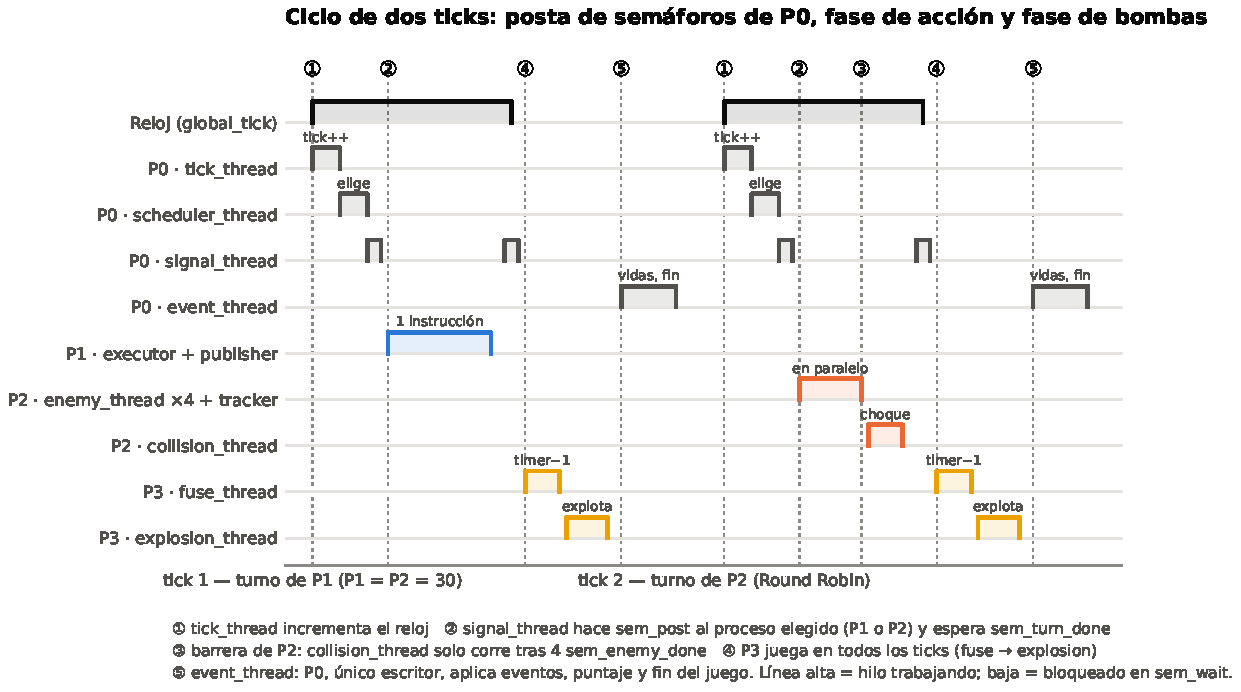
\includegraphics[width=\textwidth]{figuras/tick.pdf}
\caption{Diagrama temporal de sincronización por turnos: posta de los cuatro hilos de P0, fase de acción, barrera de P2 y fase de bombas.}
\label{fig:tick}
\end{figure}

\subsubsection{Paralelismo seguro en P2 y en P3}
En el tick 2 los cuatro \cod{enemy\_thread} y el rastreador se ejecutan en paralelo; la línea de \cod{collision\_thread} sube recién cuando el controlador recibió los cuatro \cod{sem\_enemy\_done}. En P3 ocurre lo mismo a menor escala: \cod{explosion\_thread} no arranca hasta que \cod{fuse\_thread} terminó. Así el paralelismo interno nunca expone un estado intermedio a quien lo consume.

\subsubsection{Planificación por prioridad y Round Robin}
La Figura~\ref{fig:turnos} se construyó con la salida real del programa en tres escenarios. Con las prioridades por defecto (20 y 30) P2 recibe todos los turnos. En el ejemplo 8.5 del enunciado (40 y 30) P1 juega hasta que, en T7, pide prioridad 25; P0 la aplica al inicio de T8 y desde ahí juega P2. Con prioridades iguales los turnos se alternan, y la misma secuencia de movimientos produce otro resultado: la bomba se coloca en T5, explota en T8 y Bomberman, que solo alcanzó a dar un paso, pierde una vida. El resultado de la partida depende de la planificación, no solo de los movimientos.

\begin{figure}[H]
\centering
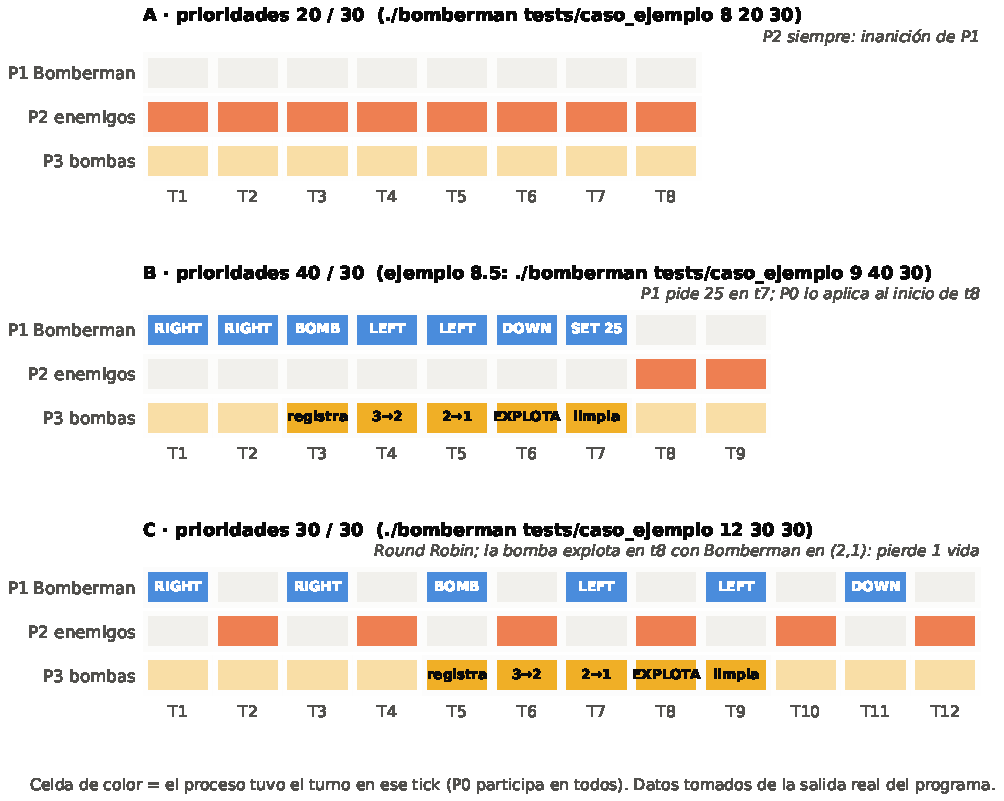
\includegraphics[width=\textwidth]{figuras/turnos.pdf}
\caption{Turnos por tick en tres escenarios de prioridad, tomados de la salida real de \cod{./bomberman}.}
\label{fig:turnos}
\end{figure}

\subsubsection{Modelo lock-step}
En ambas figuras se observa que en cada tick hay exactamente una fase de acción (P1 o P2) seguida de una fase de bombas (P3), y que P0 no avanza el reloj hasta recibir \cod{sem\_turn\_done} de cada una. Los semáforos POSIX garantizan, por tanto, una serialización cooperativa estricta entre procesos, mientras que dentro de cada proceso el paralelismo queda acotado por barreras y postas.

% =============================================================================
\section{Experimentación inicial}

\subsection{Metodología de medición}

Durante el desarrollo (cinco procesos y hasta dieciocho hilos sobre una misma memoria compartida) nos encontramos con varias condiciones de carrera. Para demostrar cada una de forma objetiva seguimos el mismo protocolo experimental.

\begin{enumerate}
  \item \textbf{Dos versiones del mismo código.} Una \emph{sin} la primitiva de sincronización, donde la carrera se manifiesta, y otra \emph{con} ella (mutex, semáforo, barrera, orden o liberación), obtenidas con una bandera de compilación (\cod{-DBUGGY}). Cada experimento es un programa corto en \cod{informe/experimentos/} que reproduce el patrón exacto de nuestro código, con los mismos nombres de hilos, semáforos y mutex.
  \item \textbf{Un parámetro medible que revele la carrera.} Según el caso: la corrección del dato compartido, las lecturas inconsistentes, los eventos perdidos, el orden de los eventos o el tiempo hasta el cierre.
  \item \textbf{Repetición masiva.} Ejecutamos cada versión entre 50 y 1000 veces y graficamos el parámetro corrida a corrida.
  \item \textbf{Señal de la carrera = no determinismo.} La versión con carrera entrega resultados distintos entre corridas (nube dispersa); la corregida entrega siempre el mismo resultado correcto (línea plana, desviación estándar 0).
  \item \textbf{Respaldo de recursos.} Además del parámetro discriminante medimos tiempo, uso de CPU y memoria máxima (MaxRSS) con \cod{/usr/bin/time}.
  \item \textbf{Amplificación de la ventana crítica.} Donde la ventana es de nanosegundos, se agrega trabajo simulado (un bucle corto) en el punto donde el código real lee un archivo o recorre una tabla, para que la carrera sea reproducible.
\end{enumerate}

\textbf{Entorno.} Ubuntu sobre WSL2 (kernel 6.18), procesador Intel Core i5-12450HX con 12 hilos lógicos, \cod{gcc} 15.2 con \cod{-O2 -pthread}. Todo el proceso es reproducible con \cod{informe/experimentos/run.sh} (corre los experimentos y guarda los CSV) y \cod{graficos.py} (genera las figuras y los números de las tablas).

Un hallazgo transversal: en cinco de las seis familias el discriminador es la \emph{corrección del dato}, no el tiempo ni la memoria. Una carrera de escritura concurrente no agota recursos: corrompe la consistencia del estado compartido. La excepción es el interbloqueo, donde el discriminador sí es el tiempo, porque el proceso defectuoso nunca termina. Como varios casos de prueba ejercitan la misma carrera en escenarios distintos, los agrupamos en seis familias según el recurso compartido y la primitiva involucrada; la correspondencia se resume en la Tabla~\ref{tab:corresp}.

\subsection{Validación de extremo a extremo con el juego real}

Antes de aislar cada carrera verificamos que el sistema completo sea determinista: ejecutamos el binario real (rama \cod{main}, commit \cod{853aa4d}) \NjuegoN{} veces en cada caso de prueba y comparamos el \emph{hash} de la salida completa (todas las líneas de P0, P1, P2 y P3, en orden). Si alguna carrera alterara el orden o el resultado de un solo tick, aparecería más de un hash distinto.

\begin{table}[H]
\centering\small
\begin{tabular}{@{}lcccclrr@{}}
\toprule
\textbf{Caso} & \textbf{máx.} & \textbf{prio.} & \textbf{corridas} & \textbf{salidas} & \textbf{resultado final} & \textbf{ms} & \textbf{MB}\\
 & \textbf{ticks} & \textbf{P1/P2} & & \textbf{distintas} & \textbf{(res./tick/vidas/score)} & & \\
\midrule
\texttt{caso\_ejemplo} & 9 & 40/30 & 300 & 1 & 1 / 9 / 3 / 20 & $<$10 & 2.0 \\
\texttt{caso\_ejemplo} & 12 & 30/30 & 300 & 1 & 1 / 12 / 2 / 20 & $<$10 & 2.1 \\
\texttt{caso\_demo} & 16 & 40/30 & 300 & 1 & 1 / 16 / 1 / 210 & $<$10 & 2.0 \\
\texttt{caso\_victoria} & 20 & 40/30 & 300 & 1 & 3 / 7 / 3 / 400 & $<$10 & 2.1 \\
\texttt{caso\_derrota} & 20 & 40/30 & 300 & 1 & 2 / 10 / 0 / 0 & $<$10 & 2.1 \\
\texttt{caso\_sin\_movimientos} & 30 & 30/30 & 300 & 1 & 4 / 6 / 3 / 0 & $<$10 & 2.0 \\
\bottomrule

\end{tabular}
\caption{Determinismo del juego completo: número de salidas distintas (por \emph{hash}) entre todas las corridas de cada caso. El resultado final es la última línea del programa; resultado 1 = máximo de ticks, 2 = derrota, 3 = victoria, 4 = sin movimientos. Tiempo medio por corrida (ms) y memoria máxima (MB).}
\label{tab:juego}
\end{table}

\NJuegoTexto

Complementariamente, compilamos con \cod{make tsan} (ThreadSanitizer) y corrimos los cinco casos: no se reportó ninguna carrera de datos entre hilos. ThreadSanitizer observa los hilos de un proceso, pero no los accesos entre procesos distintos sobre \cod{mmap}; por eso las familias siguientes se demuestran con experimentos dedicados.

% -----------------------------------------------------------------------------
\subsection{Familia 1 --- Vidas de Bomberman y regla de un solo escritor}

\textbf{La carrera que encontramos.} Al diseñar los daños, lo natural era que quien detecta el golpe restara la vida: P2 al detectar un choque y P3 al detectar fuego sobre Bomberman. Pero \cod{bomber\_lives--} es un ciclo leer--modificar--escribir; si dos procesos lo ejecutan a la vez sin exclusión, uno sobrescribe al otro y se pierde un descuento (\emph{lost update}). El caso \cod{caso\_demo} lo provoca: en el tick 5 explotan dos bombas en cadena con Bomberman dentro del fuego.

\textbf{Técnica aplicada.} Centralizar la actualización en P0 como único escritor. P2 y P3 solo publican su evento (\cod{collision\_detected}, \cod{blast\_hit\_bomber}) bajo \cod{events\_mtx}; \cod{event\_thread} los lee, descuenta como máximo una vida por tick y baja las banderas.

\textbf{Experimento.} Dos procesos hijos (P2 y P3) reportan un millón de golpes cada uno. En la versión con falla ambos hacen \cod{bomber\_lives--} directamente en la memoria compartida; en la corregida cada uno incrementa solo \emph{su} contador de eventos y P0 aplica los descuentos. \NunoN{} corridas por versión; métrica: descuentos perdidos respecto del valor correcto.

\textbf{Resultado.} Sin la solución se pierde en promedio el \NunoBugMediaPct\,\% de los descuentos (media \NunoBugMedia, rango \NunoBugMin--\NunoBugMax, $\sigma = \NunoBugSd$) y el \NunoBugPct\,\% de las corridas termina con las vidas correctas. Con la solución, el \NunoOkPct\,\% de las corridas da exactamente el valor esperado ($\sigma = 0$). $\to$ \emph{Carrera resuelta}.

\begin{figure}[H]
\centering
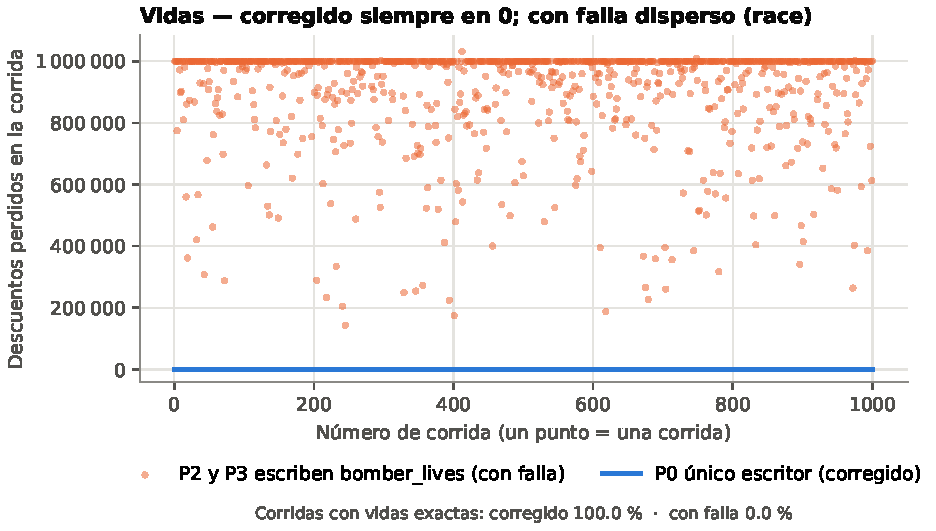
\includegraphics[width=0.92\textwidth]{figuras/f1_dispersion.pdf}
\caption{Dispersión de la familia Vidas.}
\end{figure}

\begin{figure}[H]
\centering
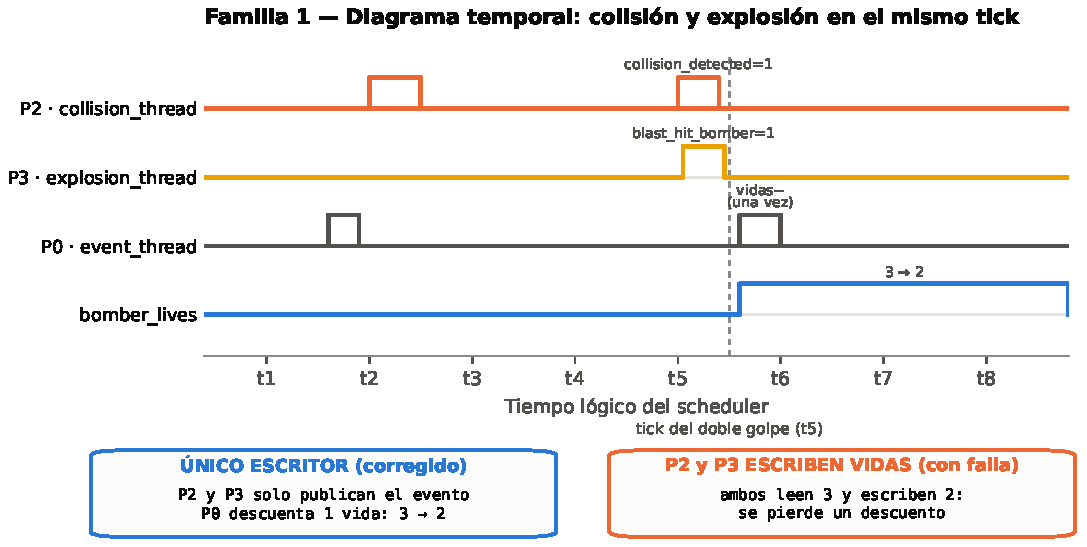
\includegraphics[width=0.92\textwidth]{figuras/f1_temporal.pdf}
\caption{Diagrama temporal de la familia Vidas: colisión y explosión en el mismo tick.}
\end{figure}

\begin{table}[H]
\centering\small
\begin{tabularx}{\textwidth}{@{}Ycccc@{}}
\toprule
\textbf{Variante} & \textbf{Corridas correctas} & \textbf{Tiempo medio (s)} & \textbf{CPU medio (\%)} & \textbf{Memoria máx.\ (KB)}\\
\midrule
P0 único escritor (corregido) & \NunoOkPct\,\% & \NunoOkTiempo & \NunoOkCpu & \NunoOkMem\\
P2 y P3 escriben (con falla) & \NunoBugPct\,\% & \NunoBugTiempo & \NunoBugCpu & \NunoBugMem\\
\bottomrule
\end{tabularx}
\caption{Métricas de la familia Vidas.}
\end{table}

\textbf{Interpretación.} Tiempo, CPU y memoria son del mismo orden en ambas versiones: los procesos hacen el mismo trabajo y ocupan lo mismo. La carrera no agota recursos, corrompe el dato; por eso lo que la delata es la exactitud de las vidas, y en la gráfica aparece como no determinismo: la versión con falla se dispersa y la corregida es una línea plana en 0. En el juego real esta regla se ve en \cod{caso\_demo}: dos explosiones en el mismo tick y una sola vida perdida (3 $\to$ 2).

% -----------------------------------------------------------------------------
\subsection{Familia 2 --- Uso correcto de semáforos en P2}

Los semáforos importan de dos formas, y nos topamos con una carrera en cada una: en el \emph{orden} (cuándo corre algo) y en la \emph{equidad} (quién atiende cada turno). A estas se suma un tercer caso, encontrado al revisar el código real.

\paragraph{(a) Orden --- barrera antes de \cod{collision\_thread}.}

\textbf{La carrera que encontramos.} Los cuatro enemigos se mueven en paralelo y luego \cod{collision\_thread} compara sus posiciones con la de Bomberman. Sin sincronización, el detector leía posiciones mientras los enemigos aún se movían: posiciones a medio actualizar y, por tanto, colisiones falsas o perdidas.

\textbf{Técnica aplicada.} Una barrera con el semáforo contador \cod{sem\_enemy\_done}: el controlador hace \cod{sem\_wait} una vez por cada enemigo vivo antes de despertar a \cod{collision\_thread}.

\textbf{Experimento.} Versión sin barrera contra versión con barrera, \NdosN{} corridas de 200 turnos cada una. Métrica: turnos en los que el detector leyó alguna posición que no era la final del turno (lectura sucia).

\textbf{Resultado.} Sin la barrera, las lecturas sucias varían entre corridas (media \NdosBugMedia, rango \NdosBugMin--\NdosBugMax, $\sigma = \NdosBugSd$): \NdosBugLimpias\,\% de corridas limpias. Con la barrera, 0 siempre: \NdosOkLimpias\,\% de corridas limpias. $\to$ \emph{Carrera resuelta}.

\begin{figure}[H]
\centering
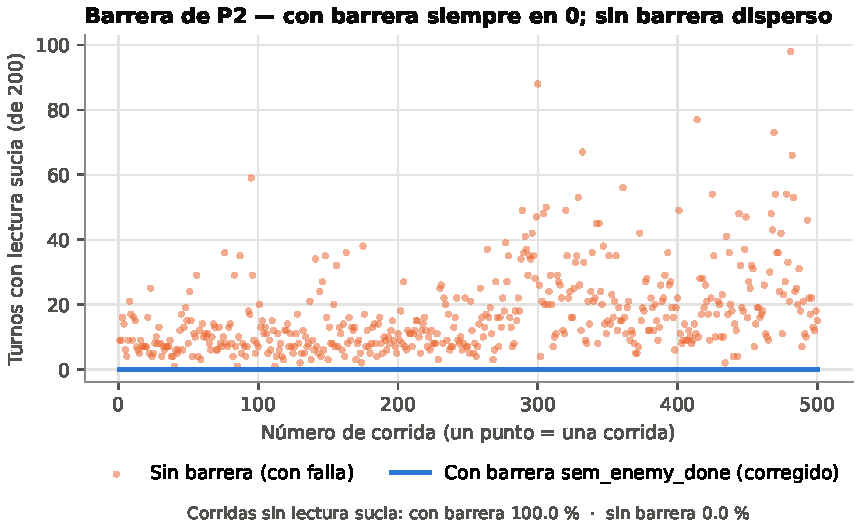
\includegraphics[width=0.92\textwidth]{figuras/f2_dispersion.pdf}
\caption{Dispersión de la familia Semáforos (barrera).}
\end{figure}

\begin{figure}[H]
\centering
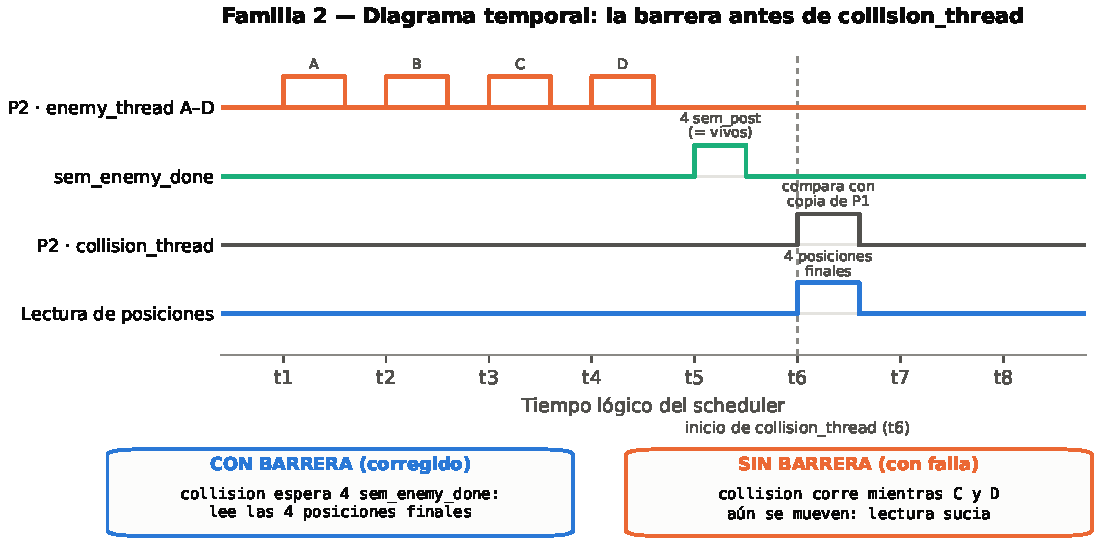
\includegraphics[width=0.92\textwidth]{figuras/f2_temporal.pdf}
\caption{Diagrama temporal de la familia Semáforos: la barrera y la lectura de posiciones.}
\end{figure}

\begin{table}[H]
\centering\small
\begin{tabularx}{\textwidth}{@{}Ycccc@{}}
\toprule
\textbf{Variante} & \textbf{Lecturas sucias (media)} & \textbf{Tiempo medio (s)} & \textbf{CPU medio (\%)} & \textbf{Memoria máx.\ (KB)}\\
\midrule
Con barrera (corregido) & 0 & \NdosOkTiempo & \NdosOkCpu & \NdosOkMem\\
Sin barrera (con falla) & \NdosBugMedia{} (rango \NdosBugMin--\NdosBugMax) & \NdosBugTiempo & \NdosBugCpu & \NdosBugMem\\
\bottomrule
\end{tabularx}
\caption{Métricas de la familia Semáforos (orden).}
\end{table}

\textbf{Interpretación.} Los recursos son del mismo orden en ambas versiones; sin la barrera el programa es incluso algo más rápido porque no espera a los hilos. Quitar la barrera no agota recursos, solo cambia el orden de ejecución. El parámetro que revela la carrera es la lectura sucia.

\paragraph{(b) Equidad --- un semáforo por enemigo.}

\textbf{La carrera que encontramos.} Si se despierta a los cuatro enemigos con un único semáforo contador posteado cuatro veces por turno, nada garantiza que cada enemigo tome exactamente una ficha: uno que ya está en CPU puede tomar dos y otro quedarse sin mover. En el juego esto significa que un enemigo ejecuta dos instrucciones en un turno y otro ninguna.

\textbf{Técnica aplicada.} Un semáforo por enemigo, \cod{sem\_start\_enemy[i]}: el controlador postea uno a cada enemigo vivo, y así cada uno atiende exactamente su turno.

\textbf{Experimento.} 25\,000 turnos por enemigo (100\,000 fichas por corrida); contamos cuántas atiende cada uno. Versión con un semáforo compartido contra versión con uno por enemigo, \NequiN{} corridas.

\textbf{Resultado.} Con el semáforo compartido el reparto es desigual y cambia en cada corrida: en la corrida mediana los enemigos atendieron \NequiRepA, \NequiRepB, \NequiRepC{} y \NequiRepD{} turnos (desbalance de \NequiRepDes, un \NequiRepPct\,\% del ideal). Sobre las \NequiN{} corridas, el desbalance (máx $-$ mín) fue en promedio \NequiBugMedia{} turnos ($\sigma = \NequiBugSd$), llegando a \NequiBugMax{} en el peor caso (un enemigo atendió \NequiPeorMax{} y otro \NequiPeorMin). Con un semáforo por enemigo los cuatro atienden exactamente 25\,000 siempre (desbalance \NequiOkMax). $\to$ \emph{Carrera resuelta}.

\begin{figure}[H]
\centering
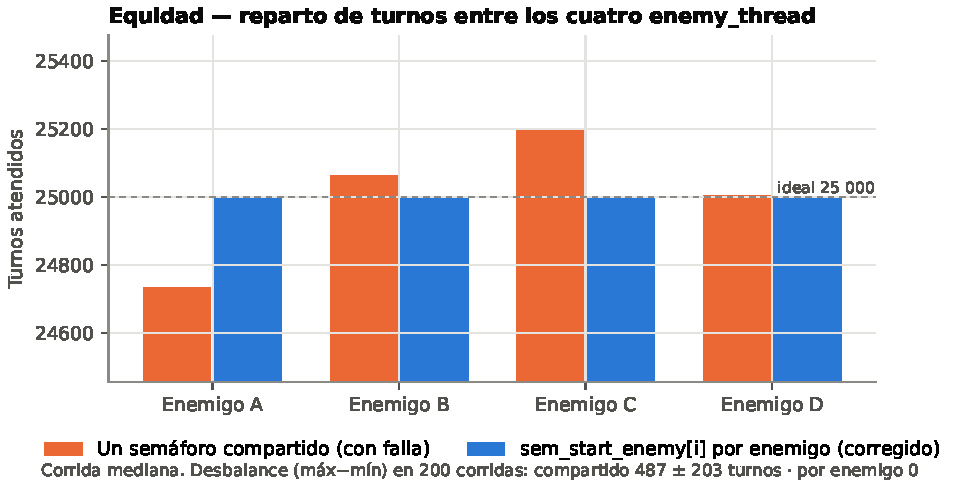
\includegraphics[width=0.92\textwidth]{figuras/f2_barras.pdf}
\caption{Turnos atendidos por cada enemigo (familia Semáforos, equidad).}
\end{figure}

\begin{table}[H]
\centering\small
\begin{tabularx}{\textwidth}{@{}Yccc@{}}
\toprule
\textbf{Variante} & \textbf{Desbalance (máx$-$mín)} & \textbf{Tiempo medio (s)} & \textbf{CPU medio (\%)}\\
\midrule
\cod{sem\_start\_enemy[i]} (corregido) & \NequiOkMax{} (exacto: 25\,000 c/u) & \NequiOkTiempo & \NequiOkCpu\\
Un semáforo compartido (con falla) & \NequiBugMedia{} en promedio (hasta \NequiBugMax) & \NequiBugTiempo & \NequiBugCpu\\
\bottomrule
\end{tabularx}
\caption{Desbalance de turnos entre enemigos.}
\end{table}

\textbf{Interpretación.} Ambas versiones hacen el mismo trabajo (100\,000 fichas), así que el costo es comparable; lo único que cambia es \emph{quién} atiende cada turno. El parámetro que revela la carrera es el reparto, no los recursos.

\paragraph{(c) Orden en el código real --- rastreador antes del detector.}

\textbf{La carrera que encontramos.} Al revisar \cod{enemy.c} notamos que, después de la barrera, \cod{enemy\_controller\_thread} despierta \emph{a la vez} a \cod{bomber\_tracker\_thread} (que copia la posición de Bomberman) y a \cod{collision\_thread} (que compara contra esa copia). Ambos usan \cod{local\_pos\_mtx}, así que no hay carrera de datos y ThreadSanitizer no reporta nada; pero si el detector toma el mutex primero, compara contra la copia del turno anterior de P2. Si Bomberman se movió entre medio, el choque se pierde o se detecta donde ya no está.

\textbf{Experimento.} Armamos un caso mínimo (\cod{experimentos/caso\_tracker}, prioridades 30/30, 2 ticks): en el tick 1 Bomberman avanza a (2,1) y en el tick 2 ---el primer turno de P2--- el enemigo A entra en esa misma celda. El choque solo se detecta si el detector usa la copia \emph{nueva} de la posición. Compilamos el \cod{enemy.c} real en tres variantes y corrimos cada una \NtrackN{} veces: tal cual está; con un retardo de 2~ms al inicio de \cod{bomber\_tracker\_thread} (amplificación); y con ese retardo más la corrección propuesta (despertar al rastreador, esperar \cod{sem\_tracker\_done} y recién entonces despertar al detector). El script es \cod{experimentos/e2c\_tracker.py}.

\textbf{Resultado.} \NTrackerTexto{} $\to$ \emph{Carrera encontrada en el código actual; corrección propuesta y verificada}.

\begin{figure}[H]
\centering
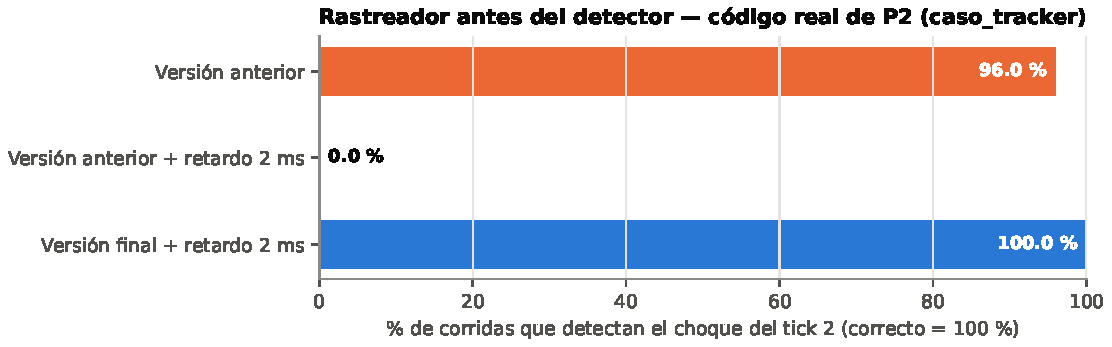
\includegraphics[width=0.92\textwidth]{figuras/f2c_barras.pdf}
\caption{Familia Semáforos, orden en el código real: porcentaje de corridas que detectan el choque.}
\end{figure}

% -----------------------------------------------------------------------------
\subsection{Familia 3 --- Orden de las fases de P3 (temporizador y explosión)}

\textbf{La carrera que encontramos.} En P3, \cod{fuse\_thread} decrementa los temporizadores y \cod{explosion\_thread} detona las bombas que llegaron a 0. Ambos hilos protegen la tabla \cod{bombs[]} con \cod{bombs\_mtx}, así que no hay carrera de datos; pero si se los despierta a la vez, \cod{explosion\_thread} puede revisar la tabla \emph{antes} del último decremento y la bomba explota un tick tarde. Es una carrera de orden que rompe la regla del juego ``una bomba pedida en $t$ explota en $t+3$'' y cambia quién queda dentro del fuego.

\textbf{Técnica aplicada.} Una posta de semáforos dentro de P3: el controlador hace \cod{sem\_post(sem\_fuse\_go)}, espera \cod{sem\_fuse\_done}, y solo entonces hace \cod{sem\_post(sem\_explosion\_go)}. El registro de bombas nuevas va al final del turno.

\textbf{Experimento.} 800 ticks por corrida colocando una bomba nueva en cuanto la anterior explota (unas \NtresBombas{} bombas por corrida); \NtresN{} corridas por versión. Métrica: bombas que explotan en un tick distinto de $t+3$.

\textbf{Resultado.} Con las fases en paralelo, en promedio \NtresBugMedia{} bombas por corrida explotan fuera de tiempo (rango \NtresBugMin--\NtresBugMax, $\sigma = \NtresBugSd$); solo el \NtresBugLimpias\,\% de las corridas queda limpio. Con la posta, \NtresOkLimpias\,\% de corridas sin ninguna bomba fuera de tiempo. $\to$ \emph{Carrera resuelta}.

\begin{figure}[H]
\centering
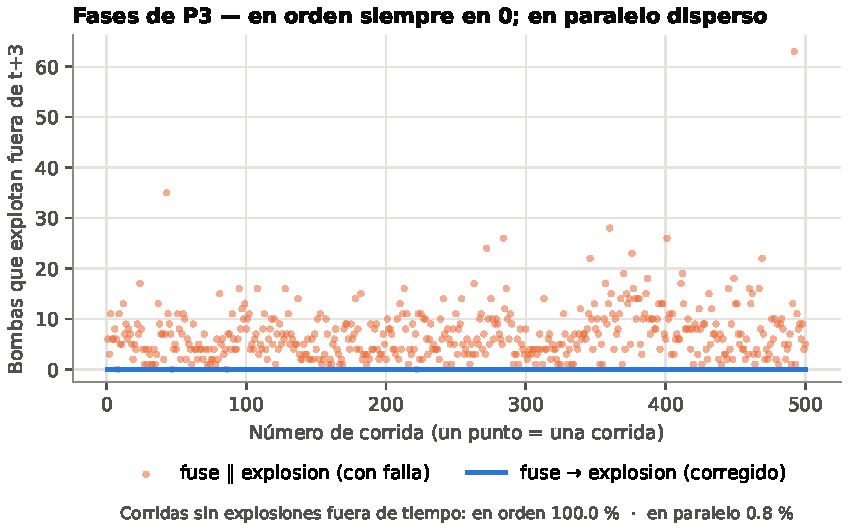
\includegraphics[width=0.92\textwidth]{figuras/f3_dispersion.pdf}
\caption{Dispersión de la familia Fases de P3.}
\end{figure}

\begin{figure}[H]
\centering
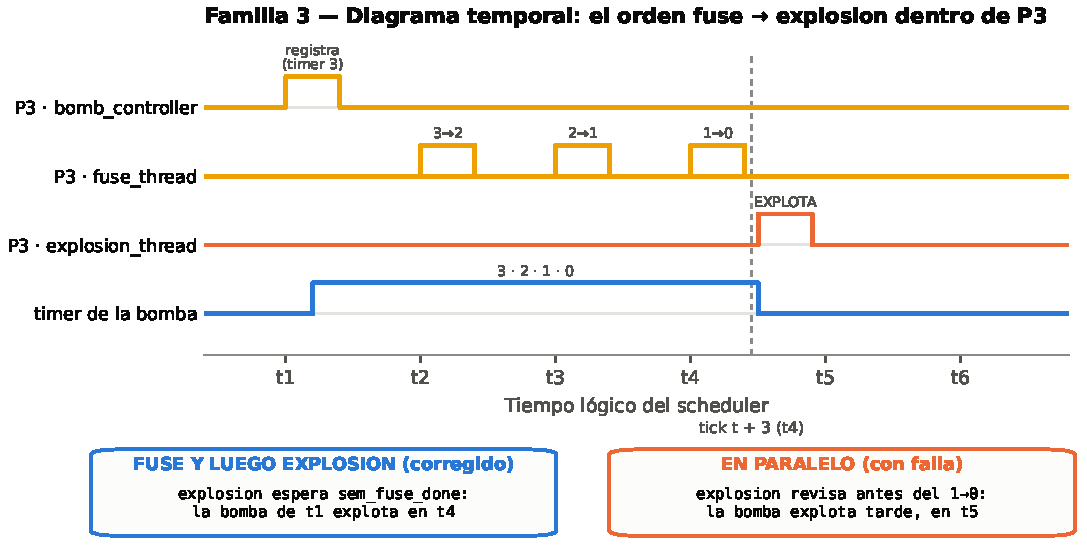
\includegraphics[width=0.92\textwidth]{figuras/f3_temporal.pdf}
\caption{Diagrama temporal de la familia Fases de P3.}
\end{figure}

\begin{table}[H]
\centering\small
\begin{tabularx}{\textwidth}{@{}Ycccc@{}}
\toprule
\textbf{Variante} & \textbf{Fuera de $t+3$ (media)} & \textbf{Tiempo medio (s)} & \textbf{CPU medio (\%)} & \textbf{Memoria máx.\ (KB)}\\
\midrule
fuse $\to$ explosion (corregido) & 0 & \NtresOkTiempo & \NtresOkCpu & \NtresOkMem\\
En paralelo (con falla) & \NtresBugMedia & \NtresBugTiempo & \NtresBugCpu & \NtresBugMem\\
\bottomrule
\end{tabularx}
\caption{Métricas de la familia Fases de P3.}
\end{table}

\textbf{Interpretación.} Esta familia muestra que un mutex no basta: protege el \emph{dato} pero no el \emph{orden}. Los recursos son prácticamente iguales; lo que cambia es el tick en que ocurre la explosión. En el juego real, \cod{caso\_ejemplo} con prioridades 40/30 registra la bomba en el tick 3 y la detona en el tick 6, y con 30/30 la registra en el 5 y la detona en el 8, siempre a $t+3$.

% -----------------------------------------------------------------------------
\subsection{Familia 4 --- Buzones entre procesos (bomba y prioridad)}

\textbf{La carrera que encontramos.} Los pedidos de P1 viajan en buzones de varios campos: \cod{bomb\_request\_x}, \cod{bomb\_request\_y} y \cod{bomb\_request\_active} para la bomba, y \cod{pending\_priority\_*} con su bandera para la prioridad. Si P3 lee el buzón mientras P1 lo escribe, puede ver una coordenada nueva junto con otra vieja (\emph{torn read}) y colocar la bomba en una celda que nadie pidió.

\textbf{Técnica aplicada.} Dos capas. Primero, el \emph{lock-step}: P1 solo escribe el buzón durante su turno y P3 solo lo lee durante el suyo, así que nunca se solapan. Segundo, el lector toma el mutex del buzón (\cod{bomb\_req\_mtx} en P3, \cod{prio\_mtx} en P0), configurado con \cod{PTHREAD\_PROCESS\_SHARED} para que funcione entre procesos. El experimento muestra qué ocurre si ambos lados acceden a la vez y cuál es la protección completa: que el escritor también tome el mutex (ver Recomendaciones).

\textbf{Experimento.} P1 (proceso hijo) escribe 200\,000 pedidos en los que siempre $x = y$; P3 (proceso padre) atiende el buzón y cuenta cuántas veces lee $x \ne y$. Versión sin mutex contra versión con mutex, \NcuatroN{} corridas. Métrica: lecturas rotas.

\textbf{Resultado.} Sin el mutex, P3 detecta en promedio \NcuatroBugMedia{} lecturas rotas por corrida (rango \NcuatroBugMin--\NcuatroBugMax, $\sigma = \NcuatroBugSd$): solo el \NcuatroBugLimpias\,\% de corridas queda limpio. Con el mutex, 0 siempre: \NcuatroOkLimpias\,\% limpias. $\to$ \emph{Carrera resuelta}.

\begin{figure}[H]
\centering
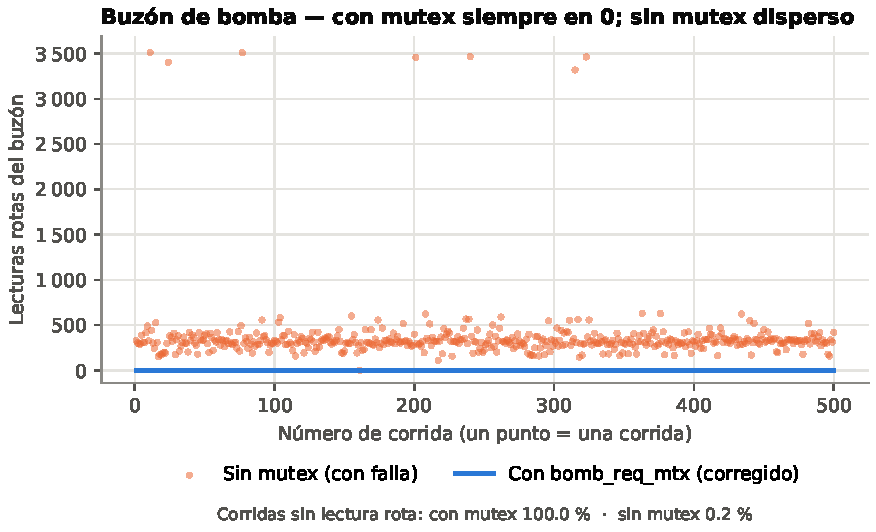
\includegraphics[width=0.92\textwidth]{figuras/f4_dispersion.pdf}
\caption{Dispersión de la familia Buzones.}
\end{figure}

\begin{figure}[H]
\centering
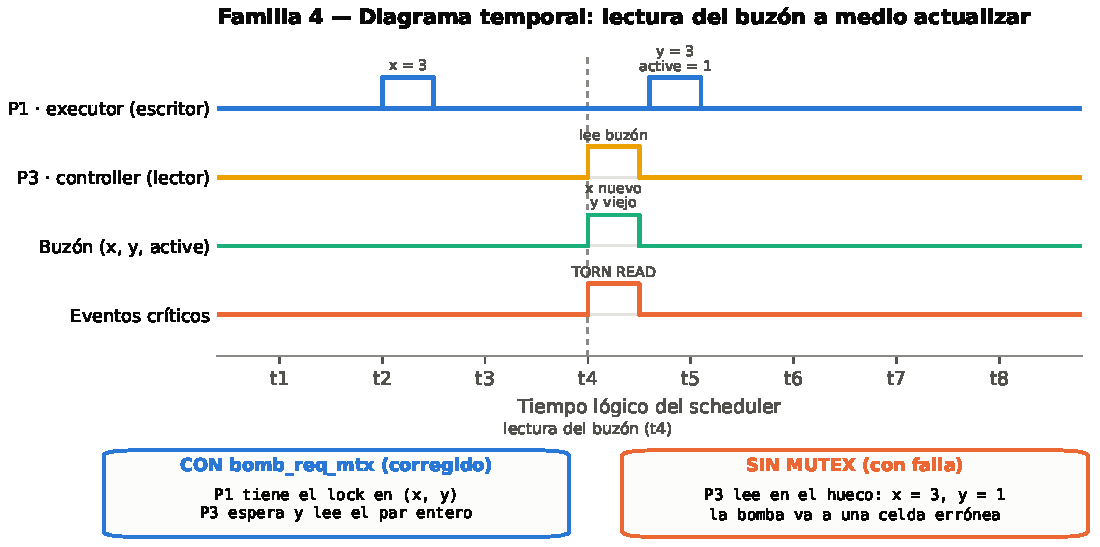
\includegraphics[width=0.92\textwidth]{figuras/f4_temporal.pdf}
\caption{Diagrama temporal de la familia Buzones: lectura a medio actualizar.}
\end{figure}

\begin{table}[H]
\centering\small
\begin{tabularx}{\textwidth}{@{}Ycccc@{}}
\toprule
\textbf{Variante} & \textbf{Lecturas rotas (media)} & \textbf{Tiempo medio (s)} & \textbf{CPU medio (\%)} & \textbf{Memoria máx.\ (KB)}\\
\midrule
Con \cod{bomb\_req\_mtx} (corregido) & 0 & \NcuatroOkTiempo & \NcuatroOkCpu & \NcuatroOkMem\\
Sin mutex (con falla) & \NcuatroBugMedia & \NcuatroBugTiempo & \NcuatroBugCpu & \NcuatroBugMem\\
\bottomrule
\end{tabularx}
\caption{Métricas de la familia Buzones.}
\end{table}

\textbf{Interpretación.} Aquí el tiempo y la CPU sí difieren, pero por un efecto colateral del mutex y no por la carrera: con el mutex los dos procesos se turnan el buzón y el escritor ya no corre libre, por lo que la corrida tarda más y usa más CPU (ambos procesos compiten por el candado). La memoria es la misma. Lo que demuestra la carrera siguen siendo las lecturas rotas. Las ventanas son de nanosegundos: en una corrida típica se rompe menos del 1\,\% de los pedidos, lo que hace a esta carrera difícil de ver jugando, pero suficiente para mandar una bomba a una celda equivocada.

% -----------------------------------------------------------------------------
\subsection{Familia 5 --- Cola productor--consumidor de P1}

\textbf{La carrera que encontramos.} En P1, \cod{movement\_reader\_thread} lee el archivo completo en microsegundos, mientras que \cod{movement\_executor\_thread} consume una instrucción por turno. La cola es circular de 100 casilleros (\cod{instruction\_queue}, \cod{q\_head}, \cod{q\_tail}). Si el lector no espera a que haya espacio, da la vuelta al buffer y sobrescribe instrucciones que todavía no se ejecutaron: con un archivo de más de 100 líneas, Bomberman se ``saltaría'' movimientos.

\textbf{Técnica aplicada.} Buffer acotado con dos semáforos contadores: \cod{sem\_espacios} (inicia en 100) y \cod{sem\_items} (inicia en 0), más \cod{queue\_mtx} para \cod{q\_head} y \cod{q\_tail}. El lector hace \cod{sem\_wait(sem\_espacios)} antes de escribir y el ejecutor \cod{sem\_post(sem\_espacios)} después de leer.

\textbf{Experimento.} El lector inserta 200\,000 instrucciones numeradas; el ejecutor las consume con un pequeño trabajo por instrucción. Versión sin \cod{sem\_espacios} contra la versión completa, \NcincoN{} corridas. Métrica: instrucciones nunca ejecutadas.

\textbf{Resultado.} Sin \cod{sem\_espacios} se pierden en promedio \NcincoBugMedia{} instrucciones por corrida (el \NcincoBugMediaPct\,\%; rango \NcincoBugMin--\NcincoBugMax, $\sigma = \NcincoBugSd$): \NcincoBugLimpias\,\% de corridas sin pérdida. Con el semáforo, 0 pérdidas siempre: \NcincoOkLimpias\,\% de corridas íntegras. $\to$ \emph{Carrera resuelta}.

\begin{figure}[H]
\centering
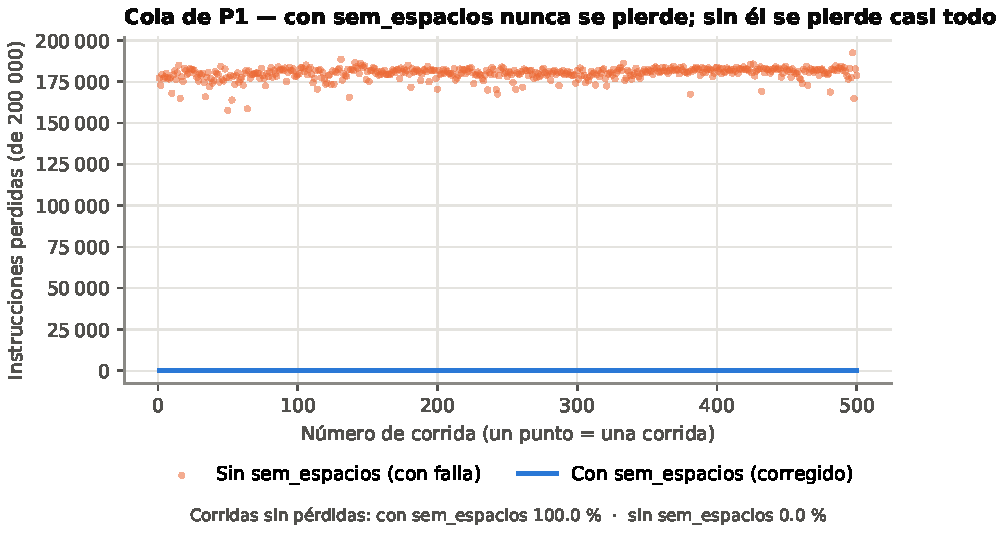
\includegraphics[width=0.92\textwidth]{figuras/f5_dispersion.pdf}
\caption{Dispersión de la familia Cola.}
\end{figure}

\begin{figure}[H]
\centering
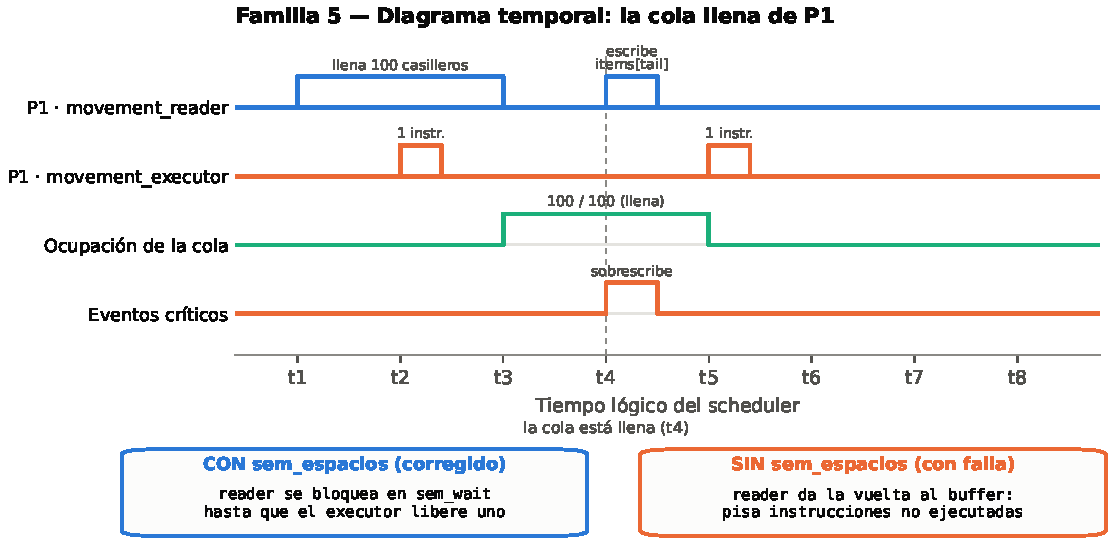
\includegraphics[width=0.92\textwidth]{figuras/f5_temporal.pdf}
\caption{Diagrama temporal de la familia Cola: el lector frente a la cola llena.}
\end{figure}

\begin{table}[H]
\centering\small
\begin{tabularx}{\textwidth}{@{}Ycccc@{}}
\toprule
\textbf{Variante} & \textbf{Instrucciones perdidas} & \textbf{Tiempo medio (s)} & \textbf{CPU medio (\%)} & \textbf{Memoria máx.\ (KB)}\\
\midrule
Con \cod{sem\_espacios} (corregido) & 0 & \NcincoOkTiempo & \NcincoOkCpu & \NcincoOkMem\\
Sin \cod{sem\_espacios} (con falla) & \NcincoBugMedia & \NcincoBugTiempo & \NcincoBugCpu & \NcincoBugMem\\
\bottomrule
\end{tabularx}
\caption{Métricas de la familia Cola.}
\end{table}

\textbf{Interpretación.} La versión con falla es incluso más rápida: el lector nunca se bloquea y termina en cuanto escribe, aunque sea encima de datos vivos. La versión correcta tarda más porque el lector y el ejecutor se alternan, que es justamente lo que se busca. Ninguno de los indicadores de hardware revela la falla; lo que la demuestra es la cantidad de instrucciones perdidas, que llega al \NcincoBugMaxPct\,\% en el peor caso.

% -----------------------------------------------------------------------------
\subsection{Familia 6 --- Cierre e interbloqueo}

\paragraph{(a) Liberación ordenada al terminar.}

\textbf{El defecto que encontramos.} Cuando el juego termina, P1, P2 y P3 están bloqueados en \cod{sem\_wait} esperando un turno que ya no llegará, y dentro de P3 los hilos \cod{fuse\_thread} y \cod{explosion\_thread} esperan su propio semáforo. Si P0 marca \cod{game\_over} y llama directamente a \cod{waitpid}, los hijos nunca despiertan para ver la bandera, y \cod{waitpid} espera para siempre: un interbloqueo. Es una falla de \emph{liveness}: el programa no se cae, se cuelga.

\textbf{Técnica aplicada.} Cierre ordenado en cadena: cada hilo de P0 pasa la posta antes de salir; \cod{signal\_thread} hace \cod{sem\_post} a \cod{sem\_bomber\_turn}, \cod{sem\_enemy\_turn}, \cod{sem\_bomb\_turn} y \cod{sem\_render}; P3 pone \cod{terminar = 1} y despierta a sus dos hilos; recién después \cod{main} llama a \cod{waitpid}.

\paragraph{(b) Orden global de adquisición de mutex.}

\textbf{El defecto que encontramos.} En una versión de P3, \cod{explosion\_thread} tomaba \cod{bombs\_mtx} $\to$ \cod{map\_mtx}, mientras que \cod{registrar\_solicitudes} (en el controlador) tomaba \cod{map\_mtx} $\to$ \cod{bomb\_req\_mtx} $\to$ \cod{bombs\_mtx}: el orden invertido de dos candados. Lo corregimos en el commit ``P3: mismo orden de mutex y regla del fuego''. El mismo riesgo existe entre procesos: \cod{explosion\_thread} de P3 y \cod{event\_thread} de P0 necesitan a la vez \cod{map\_mtx}, \cod{events\_mtx} y \cod{state\_mtx}. Si uno tiene \cod{map\_mtx} y espera \cod{events\_mtx} mientras el otro tiene \cod{events\_mtx} y espera \cod{map\_mtx}, se produce espera circular.

\textbf{Técnica aplicada.} Un orden global documentado en \cod{shared.h}: \cod{map} $\to$ \cod{bomber} $\to$ \cod{enemy} $\to$ \cod{bomb\_req} $\to$ \cod{prio} $\to$ \cod{events} $\to$ \cod{state}, respetado por todos los procesos (y la liberación en orden inverso).

\textbf{Experimento.} (a) Cuatro procesos que reproducen el \emph{lock-step} de 20 ticks y luego cierran, con y sin la liberación (\NseisAN{} corridas por versión, con un vigilante interno que interrumpe la corrida al cumplirse 1~s). (b) P0 y P3 como procesos que toman los tres mutex compartidos 20\,000 veces sin turnos (el peor caso), con el orden correcto y con el orden invertido (\NseisBN{} corridas, vigilante de 1~s). Métrica: si la corrida termina y en cuánto tiempo.

\textbf{Resultado.} (a) Con la liberación, el \NseisAOkCierra\,\% de las corridas cierra (mediana \NseisAOkMs~ms); sin ella, cierra el \NseisABugCierra\,\% y todas se interrumpen al llegar al \emph{timeout}. (b) Con el orden global, cierra el \NseisBOkCierra\,\% (mediana \NseisBOkMs~ms); con el orden invertido, el \NseisBBugCierra\,\%: los dos procesos quedan bloqueados cada uno con un candado que el otro necesita. En ambos casos la versión colgada consume casi 0\,\% de CPU, porque los procesos están dormidos en \cod{sem\_wait} o en el mutex y no girando. Presentamos la evidencia con una curva de distribución acumulada (ECDF): la versión corregida llega al 100\,\% en milisegundos y la defectuosa queda plana en 0\,\% (datos censurados por el \emph{timeout}). $\to$ \emph{Defectos resueltos}.

\begin{figure}[H]
\centering
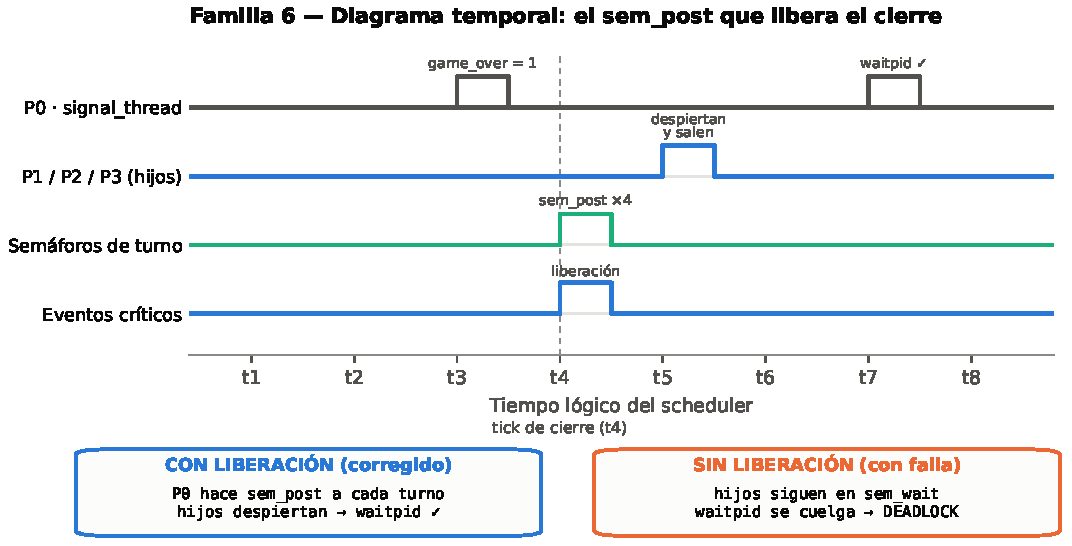
\includegraphics[width=0.92\textwidth]{figuras/f6_temporal.pdf}
\caption{Diagrama temporal de la familia Cierre: el \cod{sem\_post} que libera el cierre.}
\end{figure}

\begin{figure}[H]
\centering
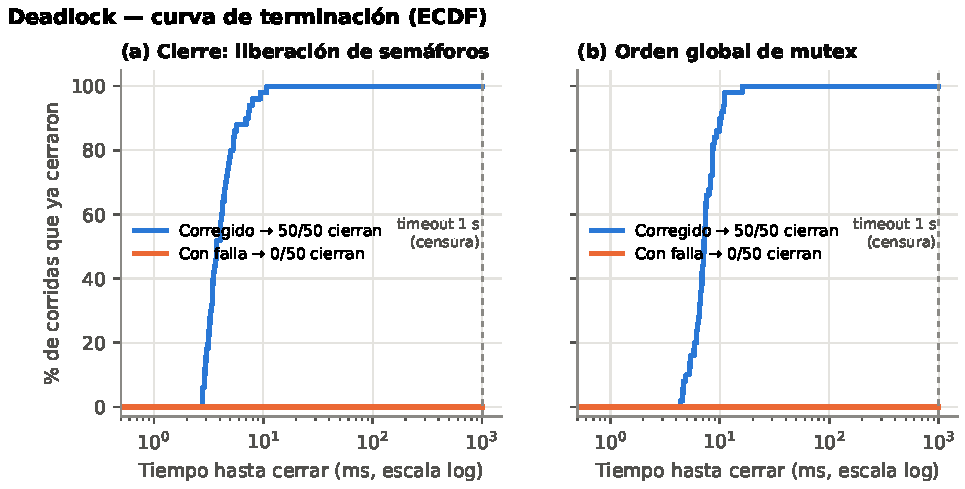
\includegraphics[width=\textwidth]{figuras/f6_ecdf.pdf}
\caption{Curva de terminación (ECDF) de la familia Cierre e interbloqueo.}
\end{figure}

\begin{table}[H]
\centering\small
\begin{tabularx}{\textwidth}{@{}Ycccc@{}}
\toprule
\textbf{Variante} & \textbf{¿Cierra?} & \textbf{Tiempo medio (s)} & \textbf{CPU medio (\%)} & \textbf{Memoria máx.\ (KB)}\\
\midrule
(a) Con liberación (corregido) & Sí (\NseisAOkCierra\,\%) & \NseisAOkTiempo & \NseisAOkCpu & \NseisAOkMem\\
(a) Sin liberación (con falla) & No (\NseisABugCierra\,\% cierran) & \NseisABugTiempo & \NseisABugCpu & \NseisABugMem\\
(b) Orden global (corregido) & Sí (\NseisBOkCierra\,\%) & \NseisBOkTiempo & \NseisBOkCpu & \NseisBOkMem\\
(b) Orden invertido (con falla) & No (\NseisBBugCierra\,\% cierran) & \NseisBBugTiempo & \NseisBBugCpu & \NseisBBugMem\\
\bottomrule
\end{tabularx}
\caption{Métricas de la familia Cierre e interbloqueo.}
\end{table}

\textbf{Interpretación.} Es la única familia en la que el discriminador directo es un recurso físico: el tiempo (milisegundos si cierra frente al segundo completo del \emph{timeout}). La CPU cercana a 0 y la memoria estable ratifican que los procesos afectados están suspendidos esperando una señal, descartando una sobrecarga del procesador. Se confirma un fallo de disponibilidad (\emph{liveness}) y no de consumo de recursos.

% -----------------------------------------------------------------------------
\subsection{Correspondencia de los casos de prueba con las familias}

La Tabla~\ref{tab:corresp} relaciona los diez escenarios de prueba del proyecto con el recurso compartido, la técnica aplicada y la familia de carreras que ejercitan. La columna ``Estado'' indica si el escenario se ejecuta con el resultado esperado en el código actual.

\begin{table}[H]
\centering\scriptsize
\begin{tabularx}{\textwidth}{@{}cp{2.6cm}p{1.35cm}p{2.0cm}YYc@{}}
\toprule
\textbf{N.º} & \textbf{Escenario} & \textbf{Familia} & \textbf{Recurso compartido} & \textbf{Técnica aplicada} & \textbf{Carrera o defecto evitado} & \textbf{Estado}\\
\midrule
1 & \cod{caso\_ejemplo 9 40 30} (ejemplo 8.5) & Fases P3, Buzones & \cod{bombs[]}, buzón de bomba y de prioridad & Posta fuse $\to$ explosion; \cod{bomb\_req\_mtx}; \cod{prio\_mtx} & Bomba fuera de $t+3$; pedido roto & Sí\\
2 & \cod{caso\_ejemplo 12 30 30} (empate) & Vidas, Fases P3 & \cod{bomber\_lives}, \cod{bombs[]} & Round Robin; P0 único escritor & Vida mal descontada al explotar en T8 & Sí\\
3 & \cod{caso\_ejemplo 8 20 30} (inanición) & Buzones & Prioridades vigentes & P0 aplica los pedidos al inicio del tick & Decisión de turno inconsistente & Sí\\
4 & \cod{caso\_demo 16 40 30} & Vidas, Semáforos, Fases P3 & \cod{bomber\_lives}, \cod{enemy\_x/y[]}, \cod{map\_grid} & Máx.\ 1 vida por tick; barrera \cod{sem\_enemy\_done}; cadena & Doble descuento; colisión con posiciones viejas & Sí\\
5 & \cod{caso\_victoria 20 40 30} & Vidas, Cierre & \cod{enemy\_alive[]}, \cod{score} & P0 único escritor; liberación ordenada & Enemigo contado dos veces; cierre colgado & Sí\\
6 & \cod{caso\_derrota 20 40 30} & Vidas, Cierre & \cod{bomber\_lives}, \cod{game\_over} & P0 único escritor; liberación ordenada & Vidas negativas; hijo bloqueado & Sí\\
7 & \cod{caso\_sin\_movimientos 30 30 30} & Cola, Cierre & Cola de P1, \cod{*\_moves\_done} & \cod{sem\_items}/\cod{sem\_espacios}; fin por EOF coordinado por P0 & Instrucción perdida; espera indefinida & Sí\\
8 & \cod{make test} (parser, 12 pruebas) & Cola & Entrada de P1 y P2 & Línea inválida no entra como turno & Turno gastado por una línea inválida & Sí\\
9 & \cod{make tsan} (5 casos) & Semáforos, Fases P3, Cola & Datos internos de P0--P3 & Mutex locales y postas & Carrera de datos entre hilos & Sí\\
10 & \cod{-r} (renderer P4) & Buzones, Cierre & Estado completo, \cod{sem\_render} & Foto con mutex en orden; \cod{sem\_render} en el cierre & Dibujo de un estado a medio cambiar; P4 colgado & Sí\\
\bottomrule
\end{tabularx}
\caption{Correspondencia de los diez escenarios de prueba con sus familias y soluciones.}
\label{tab:corresp}
\end{table}

\textbf{En síntesis:} los diez escenarios se explican a través de seis familias de carreras detectadas durante el desarrollo. Cada una se demostró empíricamente contrastando la versión desprotegida con la protegida, y se resolvió con la primitiva adecuada. Las familias Semáforos y Cierre incluyen subcasos adicionales (equidad, orden en el código real y orden de mutex), lo que totaliza nueve experimentos de sincronización documentados más la validación de extremo a extremo.

% =============================================================================
\section{Conclusiones}

\subsection{Qué se construyó}

Construimos un Bomberman, pero el objetivo real no era el juego, sino aprender a coordinar varios programas que se ejecutan al mismo tiempo sobre una misma información sin que se estorben entre sí. Es como una cocina en la que varios cocineros escriben en una única pizarra de pedidos: si dos escriben a la vez, la pizarra queda ilegible. En computación ese error se llama \emph{condición de carrera} y es el problema central del proyecto.

Repartimos el trabajo en cinco ``empleados'' independientes, llamados procesos: un árbitro (P0) que marca el ritmo del juego y es el único autorizado a modificar los datos importantes (vidas, enemigos vivos, puntaje y fin de la partida); un proceso que mueve a Bomberman (P1); otro que mueve a los cuatro enemigos y detecta los choques (P2); otro que se encarga de las bombas, el fuego y el mapa (P3); y, como extra, uno que dibuja todo en pantalla (P4). Dentro de cada proceso, tareas más pequeñas llamadas hilos trabajan en paralelo. Todos comparten una única ``pizarra'' (la memoria compartida) y, para que nadie la corrompa, usamos dos tipos de ``candados'' de POSIX: los mutex (como un baño con llave: solo entra uno a la vez) y los semáforos (como un semáforo de tránsito que reparte los turnos). La regla primaria es que cada dato tiene un solo dueño que lo escribe; los demás solo dejan pedidos o avisos. Esa sola decisión elimina de raíz la mayoría de los errores de coordinación.

\subsection{Síntesis técnica}

El proyecto implementó Bomberman como un sistema concurrente real ---cuatro procesos (\cod{fork}) más un renderer opcional, dieciocho hilos (\cod{pthread}), memoria compartida (\cod{mmap}), cinco semáforos entre procesos, siete mutex con \cod{PTHREAD\_PROCESS\_SHARED} y semáforos locales en cada proceso--- y sobre esa base identificó, demostró y resolvió las condiciones de carrera que aparecen al coordinar varios flujos sobre un estado común. El mérito técnico central no fue ``hacer que el juego funcione'', sino definir una autoridad única del estado global: P0. P1, P2 y P3 solo publican hechos (posiciones, pedidos, colisiones, explosiones) y P0 decide sus consecuencias. Las carreras que quedan se cierran con la primitiva adecuada a cada recurso: mutex para las estructuras de varios campos, barreras y postas de semáforos para el orden, un semáforo por receptor para el reparto justo, un buffer acotado con dos semáforos para la cola, un orden global de mutex y una liberación ordenada para evitar el interbloqueo.

Sobre la experimentación, el principio fue uno solo: una condición de carrera se delata por el no determinismo. La versión sin la primitiva entrega resultados distintos en cada corrida; la corregida, siempre el mismo resultado correcto (desviación estándar cero). El juego completo cumple ese criterio: todas las corridas de cada caso de prueba producen exactamente la misma salida. Un aprendizaje transversal fue elegir el parámetro correcto: en casi todas las familias el discriminador es la corrección del dato y no el tiempo ni la memoria; solo en el interbloqueo la evidencia es el tiempo, porque el proceso defectuoso nunca termina y consume casi 0\,\% de CPU al quedar dormido.

No todas las carreras fueron igual de graves. La cola de P1 sin \cod{sem\_espacios} pierde la gran mayoría de las instrucciones y los dos interbloqueos cuelgan el 100\,\% de las corridas: son fallas totales. El contador de vidas, las fases de P3 y los buzones producen datos incorrectos sin que el programa se caiga, el tipo de error más difícil de detectar. El reparto con un semáforo compartido es el más leve. La lección más fina vino de las carreras de \emph{orden} (barrera de P2, posta de P3 y rastreador antes del detector): ahí todos los datos están protegidos por mutex, ThreadSanitizer no reporta nada, y aun así el resultado puede ser incorrecto. De hecho, la única carrera que seguía activa en el código (el rastreador y el detector de P2 despertados a la vez) es de este tipo: pasó la validación de los casos de prueba y ThreadSanitizer, y solo apareció al diseñar un caso que la ejercitara, donde pierde el choque en el \NtrackRealPierde\,\% de las corridas. Un mutex protege el dato; solo un semáforo bien ubicado protege el orden.

Es importante aclarar el alcance del método: las variantes con carrera se construyeron deliberadamente quitando la primitiva con una bandera de compilación, para observar la falla y contrastarla con la versión protegida; es la forma estándar de demostrar que una primitiva es necesaria. Reconocemos también su límite: cientos de corridas dan alta confianza, pero no cubren todos los entrelazados posibles del planificador, por lo que reforzamos cada carrera con amplificación de la ventana crítica para volverla reproducible.

\subsection{Recomendaciones}

\begin{itemize}
  \item \textbf{Rastreador antes del detector en P2.} Despertar a \cod{bomber\_tracker\_thread}, esperar \cod{sem\_tracker\_done} y recién entonces despertar a \cod{collision\_thread} (Familia 2c). Es la única carrera que encontramos activa en el código actual: sin amplificación, el \NtrackRealPierde\,\% de las corridas del caso mínimo pierde el choque. La corrección es intercambiar dos líneas en \cod{enemy\_controller\_thread} y la verificamos con el mismo experimento.
  \item \textbf{Usar los mutex compartidos también del lado del escritor.} Hoy \cod{enemy\_thread} escribe \cod{enemy\_x/y} con un mutex local (\cod{local\_pos\_mtx}) en lugar de \cod{enemy\_mtx}; P1 escribe \cod{bomber\_x/y} y el buzón de bomba sin \cod{bomber\_mtx} ni \cod{bomb\_req\_mtx}; y P2 deja su pedido de prioridad con un mutex local en lugar de \cod{prio\_mtx}. El \emph{lock-step} hace que nadie lea esas variables en ese momento, pero tomar el mutex compartido haría que la corrección no dependa de la planificación (Familia 4), por ejemplo si en el futuro el renderer leyera durante un turno.
  \item \textbf{Integrar la versión con hilos de P1 en \cod{main}.} La versión de tres hilos de P1 está en la rama \cod{p1-abigail}; la probamos integrada con el resto y produce los mismos resultados en los cinco casos.
  \item \textbf{Verificación entre procesos.} ThreadSanitizer no observa la memoria compartida entre procesos; para esos accesos recomendamos mantener los experimentos de este informe como pruebas de regresión (\cod{run.sh}).
\end{itemize}

% =============================================================================
\section{Referencias}

\begin{itemize}[leftmargin=*,label=\textbullet]
  \item Coffman, E. G., Elphick, M., \& Shoshani, A. (1971). System deadlocks. \emph{ACM Computing Surveys}, 3(2), 67--78. \url{https://doi.org/10.1145/356586.356588}
  \item Downey, A. B. (2016). \emph{The Little Book of Semaphores} (2.ª ed.). Green Tea Press. \url{https://greenteapress.com/wp/semaphores/}
  \item Jagdale, D. (2021). Finite State Machine in Game Development. \emph{International Journal of Advanced Research in Science, Communication and Technology}, 10(1), 384--390. \url{https://doi.org/10.48175/IJARSCT-2062}
  \item Serebryany, K., \& Iskhodzhanov, T. (2009). ThreadSanitizer: data race detection in practice. En \emph{Proceedings of the Workshop on Binary Instrumentation and Applications (WBIA '09)} (pp. 62--71). ACM. \url{https://doi.org/10.1145/1791194.1791203}
  \item Shene, C.-K. (2002). Multithreaded programming can strengthen an operating systems course. \emph{Computer Science Education}, 12(4), 275--299. \url{https://pages.mtu.edu/~shene/PUBLICATIONS/2002/os.pdf}
  \item Silberschatz, A., Galvin, P. B., \& Gagne, G. (2018). \emph{Operating System Concepts} (10.ª ed.). Wiley.
  \item Stevens, W. R., \& Rago, S. A. (2013). \emph{Advanced Programming in the UNIX Environment} (3.ª ed.). Addison-Wesley.
  \item Tanenbaum, A. S., \& Bos, H. (2015). \emph{Modern Operating Systems} (4.ª ed.). Pearson.
\end{itemize}

\end{document}
